%%%%%%%%%%%%%%%%%%%%%%% file template.tex %%%%%%%%%%%%%%%%%%%%%%%%%
%
% This is a general template file for the LaTeX package SVJour3
% for Springer journals.          Springer Heidelberg 2010/09/16
%
% Copy it to a new file with a new name and use it as the basis
% for your article. Delete % signs as needed.
%
% This template includes a few options for different layouts and
% content for various journals. Please consult a previous issue of
% your journal as needed.
%
%%%%%%%%%%%%%%%%%%%%%%%%%%%%%%%%%%%%%%%%%%%%%%%%%%%%%%%%%%%%%%%%%%%
%

\RequirePackage{fix-cm}
%
%\documentclass{svjour3}                     % onecolumn (standard format)
%\documentclass[smallcondensed]{svjour3}     % onecolumn (ditto)
%\documentclass[smallextended]{svjour3}       % onecolumn (second format)
\documentclass[natbib, twocolumn]{svjour3}          % twocolumn
%
\smartqed  % flush right qed marks, e.g. at end of proof
%
\usepackage{graphicx}
\usepackage{changes}
\usepackage{amssymb}
\usepackage{graphicx}
\usepackage{amsmath,amssymb,latexsym,float,epsfig,subfigure}
\usepackage{mathtools, bbm}
\usepackage{amsmath} % assumes amsmath package installed
\usepackage{amssymb}  % assumes amsmath package installed
\usepackage{lipsum}
\usepackage[export]{adjustbox}
\usepackage[normalem]{ulem} % underline
\usepackage{wrapfig}
\usepackage{multirow}
\usepackage{balance}
\usepackage{color}
\usepackage{url}
\usepackage{microtype}
\usepackage{algorithm, algorithmic}
\usepackage{breqn}
\usepackage[bottom]{footmisc}


\newcommand{\argmax}{\arg\!\max}
\newcommand{\norm}[1]{\left\lVert#1\right\rVert}
\definechangesauthor{de}

 \journalname{Autonomous Robots}
%
\begin{document}

\title{Disambiguation of Human Intent Through Control Space Selection\thanks{This material is based upon work supported by the National Science Foundation under Grant CNS 1544741. Any opinions, findings and conclusions or
	recommendations expressed in this material are those of the authors and do
	not necessarily reflect the views of the aforementioned institutions.}
}
\subtitle{}


\author{Deepak E. Gopinath$^*$      \and
        Brenna D. Argall %etc.
}

\institute{ Deepak E. Gopinath \at
            Department of Mechanical Engineering,\\
            Northwestern University, Evanston, IL\\
            Shirley Ryan AbilityLab, Chicago, IL.\\
            Phone No: +1 2013109061\\
              \email{deepakgopinath@u.northwestern.edu}           %  \\
%             \emph{Present address:} of F. Author  %  if needed
           \and
           Brenna D. Argall \at
           Department of Mechanical Engineering, Department of Electrical Engineering and Computer Science, Northwestern University, Evanston, IL.\\
           Department of Physical Medicine and Rehabilitation, Northwestern University, Chicago, IL,\\
           Shirley Ryan AbilityLab, Chicago, IL.\\
           \email{brenna.argall@northwestern.edu}
           \and
           $*$ Corresponding Author
}

\date{Received: date / Accepted: date}
% The correct dates will be entered by the editor


\maketitle
\begin{abstract}
Assistive shared-control have the potential to transform the lives of millions of people afflicted with severe motor impairments as a result of spinal cord or brain injuries. The effectiveness and usefulness of shared-control robots is closely related to their ability to infer the user's needs and intentions and is often a limiting factor for providing appropriate assistance quickly, confidently and accurately. The contributions of this paper are three-fold: first, we propose a goal disambiguation algorithm which enhances the intent inference and assistive capabilities of a shared-control assistive robotic arm. Second, we introduce a novel intent inference algorithm that works in conjunction with the disambiguation scheme, inspired by \textit{dynamic field theory} in which the time evolution of the probability distribution over goals is specified as a dynamical system. Third, we present a pilot human subject study to evaluate the efficacy of the disambiguation system. This study was performed with eight subjects. Our results suggest that (a) the disambiguation system has a greater utility value as the control interface becomes more limited and the task becomes more complex, (b) subjects demonstrated a diverse range of disambiguation request behavior with a greater concentration in the earlier parts of the trial and (c) there are no differences in the onset of robot assistance between different mode switching paradigms across tasks or across interfaces. 
%\added{Add a sentence regarding subjective preferences via questionnaire here?}
\keywords{Shared Autonomy \and Intent Inference \and Intent Disambiguation \and Assistive Robotics}
% \PACS{PACS code1 \and PACS code2 \and more}
% \subclass{MSC code1 \and MSC code2 \and more}
\end{abstract}

\section{Introduction}\label{sec:intro}

Assistive and rehabilitation machines---such as robotic arms and smart wheelchairs---have the potential to transform the lives of millions of people with severe motor impairments~\citep{laplante1992assistive}. These machines can promote independence, boost self-esteem and help to extend the mobility and manipulation capabilities of such individuals, and revolutionize the way motor-impaired people interact with society~\citep{scherer1996outcomes, huete2012personal}. With rapid technological strides in the domain of assistive robotics, the machines have become more capable and complex, and with this complexity the control of these machines has become a greater challenge. 

The control of an assistive machine is typically enacted through a control interface. Moreover, the greater the motor impairment of the user, the more limited are the interfaces available for them to use. These interfaces (for example, sip-and-puffs and switch-based head arrays) are low-dimensional, discrete interfaces that can operate only in subsets of the entire control space~\citep{simpson2008tooth, nuttin2002selection}. 
The dimensionality mismatch between the control interfaces and the controllable degrees-of-freedom (DoF) of the assistive robot necessitates the partitioning of the entire control space into smaller subsets called \textit{control modes}. Moreover, the more limited and lower-dimensional the control interface, the greater the number of control modes. 
\begin{figure*}[t!]
	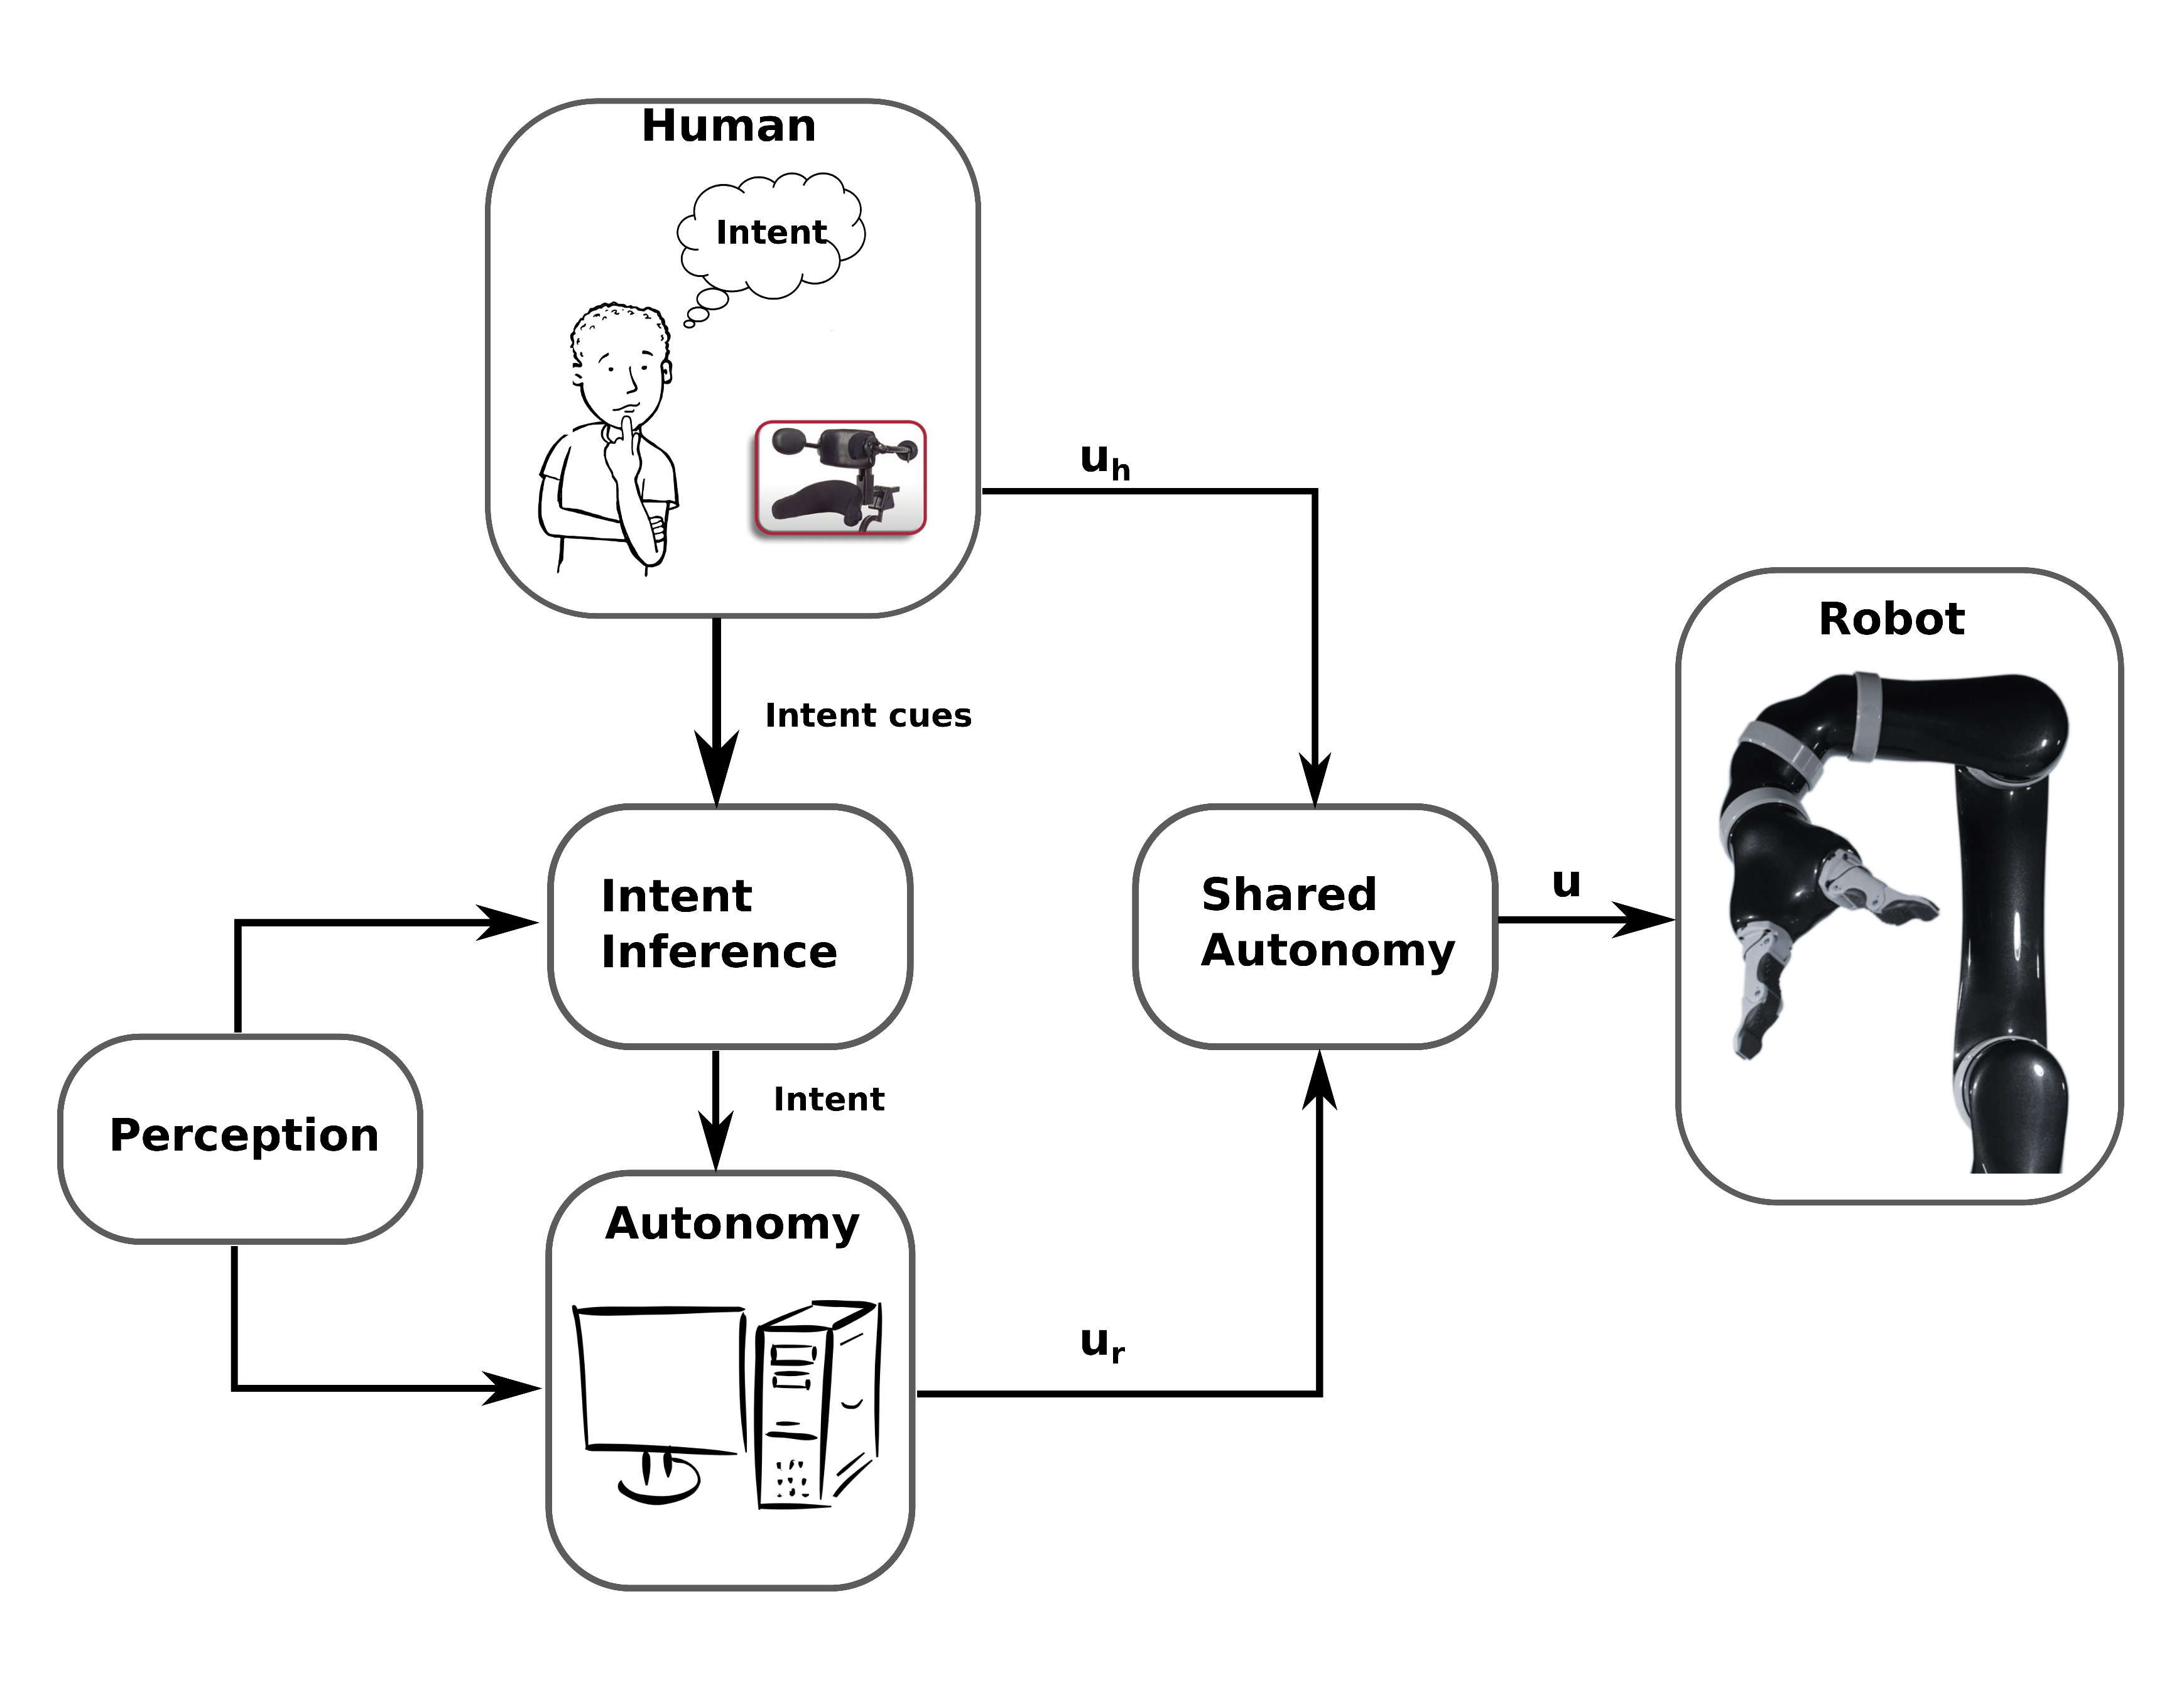
\includegraphics[keepaspectratio, width = 0.85\textwidth, center]{Fig1.eps}
	\caption{Illustration of the core components of a shared control architecture. $\boldsymbol{u}_h$ denotes the human control command, $\boldsymbol{u}_r$ denotes the autonomy control command and $\boldsymbol{u}$ is the final control command issued to the robot. The intent inference module can extract intent cues from the human in multiple ways, for example via the human control actions or biometric measures that indicate the cognitive and physical load of the user during task execution. In our work we intentionally restrict this to be similar to operating the machine without autonomy and so intent information is $\boldsymbol{u}_h$ exclusively. }
	\label{fig:shared_control}
\end{figure*}
In order to achieve full control of the machine, the user must switch between the control modes, which is referred to as \textit{mode switching} or \textit{modal control}. Mode switching adds to the cognitive and physical burden of task execution and has a detrimental effect on the performance~\citep{eftring1999technical}. 

The introduction of \textit{shared autonomy} to these assistive machines seeks to alleviate some of these issues. In a shared control system the task responsibility is shared between the user and the robot, with the aim of reducing human effort in achieving a goal. Shared autonomy systems arbitrate between the human control commands and the autonomous control commands using different strategies depending on the task context, user preference and robotic platform. Figure~\ref{fig:shared_control} depicts the key components of a typical shared control architecture and how they interact with each other.

Any assistive robotic system needs to have a good idea of the user's needs and intentions. Therefore, \textit{intent inference} is a necessary and crucial component to ensure appropriate assistance. In assistive robotic manipulation specifically, often the first step of a manipulation task is to reach for and grasp discrete objects in the environment. Intent inference therefore can be framed as a problem of estimating a probability distribution of intent likelihood over all possible goals (objects) in the environment. This inference is usually informed by various cues from the human and the environment, such as the human control actions, biometric measures and task-relevant features such as robot and goal locations. With a greater number of sensor modalities available, it is likely that the intent inference becomes more accurate. 

However, in the assistive domain, user acceptance and adoption is of paramount importance. Adding more sensors to track biometric data and object locations can become expensive and cumbersome (e.g. if the sensor must be worn by the user). For reasons of user adoption and cost, we intentionally design our assistance add-ons to be as invisible and close to the manual system as possible. As a result the intent inference is exclusively informed by the human's control commands issued to the assistive machine. The low-dimensionality, sparsity and noise in these control commands make the inference task even harder, prompting the need for robust intent inference formalisms. 

Our key insight is that certain control commands issued by the human are \textit{more intent expressive} than others, and may help the autonomy in inference accuracy. This is the notion of \textit{inverse legibility}~\citep{gopinath2017mode} in which human-generated actions \textit{help the robot} to infer the human's intent unambiguously. Consider the hypothetical reaching experiment illustrated in Figure~\ref{fig:disamb}. Since the spatial locations of the goals are maximally spread along the horizontal axis, any human control command issued along the horizontal dimension conveys a lot of information about the intended goal to the robot. In other words, motion along $x$ is more \textit{intent expressive} and will help the robot to draw accurate inference more quickly and confidently.

In this work, we investigate how the selection of a subset of the operational control dimensions/modes improves the intent inference and disambiguation capabilities of the robot. As our primary contribution we develop a control mode selection paradigm which selects the control mode in which a user-initiated motion will \textit{maximally disambiguate }human intent by eliciting more \textit{intent expressive} control commands from the user.  Furthermore, the disambiguation power of the algorithm is closely linked to, and is dependent on, the success and accuracy of the underlying intent inference mechanism~\citep{gopinath2017mode}. Therefore, as our secondary contribution, we also develop a novel intent inference scheme which utilizes ideas from \textit{dynamic field theory} that casts the time-evolution of the probability distribution over goals as a dynamical system. By doing so, the distribution evolves in continuous time and information from past states can be easily incorporated using a time-scale parameter and thereby improves the performance of the disambiguation algorithm.
%More specifically on how well past cues are incorporated into the inference process.

In Section~\ref{sec:related-work} we present an overview of relevant research in the areas of shared autonomy in assistive robotics, types of shared autonomy assistance paradigms, intent inference and synergies in human-robot interaction. Section~\ref{sec:ma} presents the mathematical formalism developed for intent inference and disambiguation. Section~\ref{sec:shared-control} focuses on the implementation details of the shared control system. The study design and experimental methods are discussed in Section~\ref{sec:ed} followed by results in Section~\ref{sec:results}. Discussion and conclusions are presented in Sections~\ref{sec:discussions} and~\ref{sec:conclusions} respectively. 
\begin{figure}
	\begin{center}
		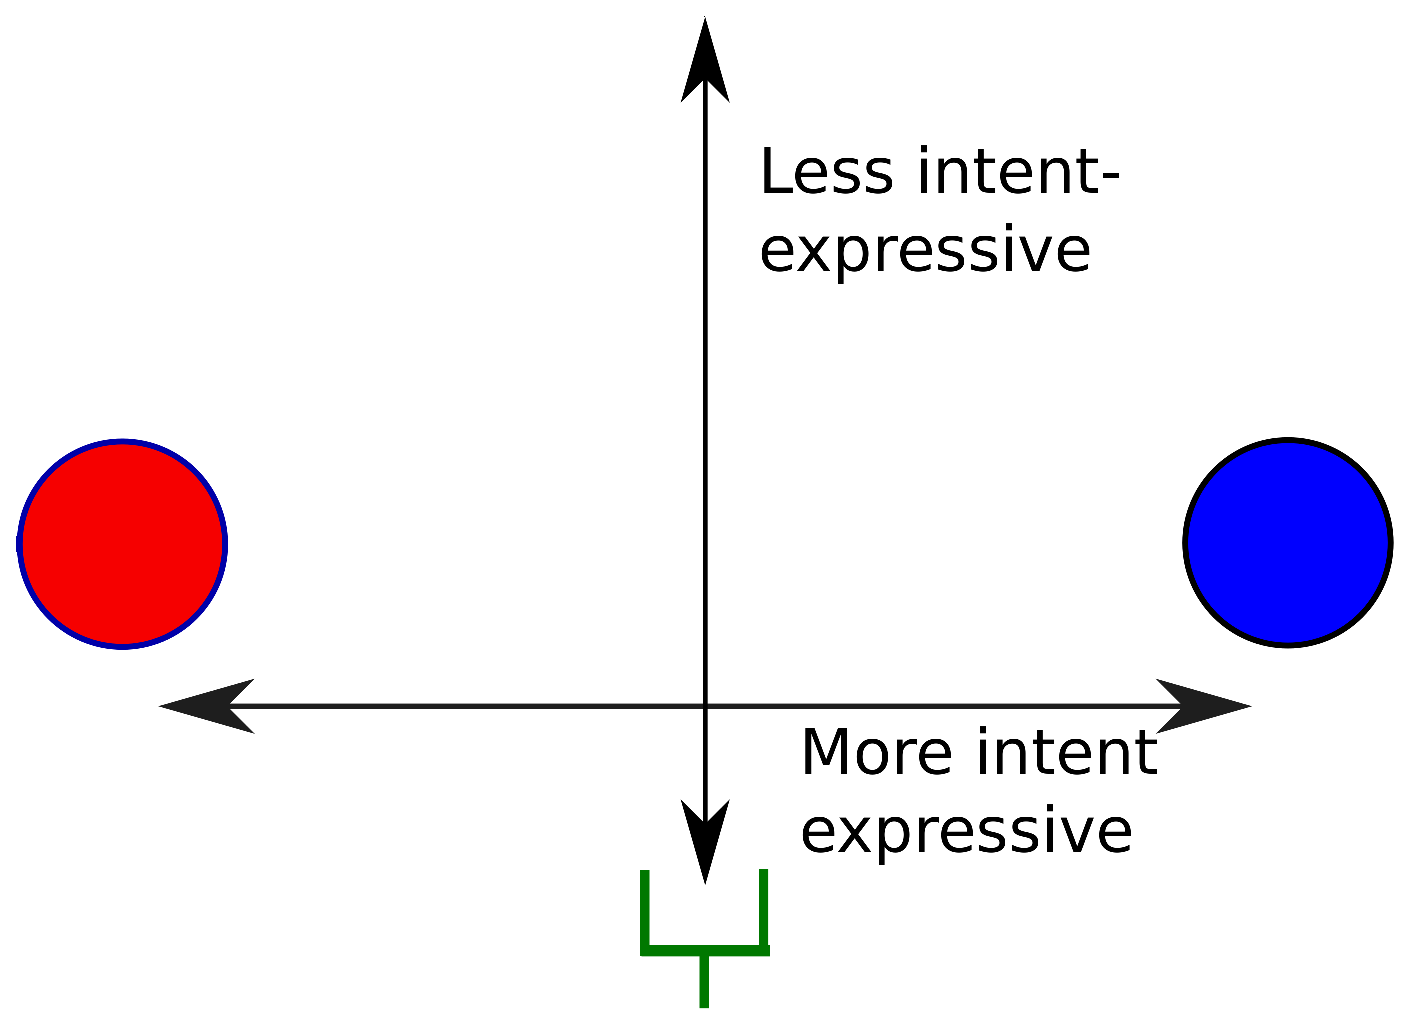
\includegraphics[width=0.35\textwidth]{Fig2.eps}
	\end{center}
	%	\vspace{-.45cm}
	\caption{Illustration of goal disambiguation along various control dimensions. Any motion of the end effector (green) along the y-axis will not help the system to disambiguate the two goals (A and B). However, motion along the x-axis provides cues as to which goal.}
	\label{fig:disamb}
\end{figure}


%%Understanding intent is critical. Why? Shared intention in human-human teams. Human-robot teams. Different types of paradigms exist for the same. 
%
%But we have human-in-th-loop. If the robot can elicit more intent expressive actions from the user, the inference problem becomes easier for the robot. Therefore the intent disambiguation system. 


\section{Related Work}\label{sec:related-work}
This section provides an overview of related research in the domains of shared autonomy in assistive robotics, robot assistance for modal control, intent inference in human-robot interaction and information acquisition in robotics. 

Shared-autonomy in assistive systems aims to reduce the user's cognitive and physical burden during task execution without having the user relinquish complete control~\citep{philips2007adaptive, demeester2008user, gopinath2017human, muelling2017autonomy}. The most common strategies to share control between the user and the assistive system include (a) hierarchical paradigms in which the higher level goals are entrusted with the user and the autonomy generates low-level control~\citep{tsui2011want, kim2010relationship, kim2012autonomy}, (b) control allocation in distinct partitions of the control space~\citep{driessen2005collaborative} and (c) blending user controls and robot autonomy commands~\citep{downey2016blending, storms2014blending, muelling2017autonomy}. 

In order to offset the drop in task performance due to shifting focus (\text{task switching}) from the task at hand to switching between different control modes different mode switch assistance paradigms have been proposed. For example, a simple time-optimal mode switching scheme has shown to improve task performance~\citep{herlant2016assistive, pilarski2012dynamic}. 


Shared control systems often require a good estimate of the human's intent---for example, their intended reaching target in a manipulation task or a target location in the environment in a navigation task~\citep{liu2016goal}. Intent can either be explicitly communicated by the user~\citep{choi2008laser} or can be inferred from their control signals or sensor data using various algorithms. 

Intent recognition and inference are actively studied by cognitive scientists and roboticists and can be broadly categorized into two main classes: model-based approaches and heuristic approaches. In model-based approaches, intent inference is typically cast within a Bayesian framework, and the posterior distribution over goals (belief) at any time is determined by the iterative application of Bayes theorem. Evidence in this context can be derived from a combination of factors such as task-relevant features in the environment, trajectory information, human control actions or biometric data from the user. Within the context of shared autonomy based teleoperation a Bayesian scheme for user intent prediction is used~\citep{dragan2012formalizing, javdani2017shared, admoni2016predicting} in which the user is modeled within the Markov Decision Process framework and is typically assumed to be noisily optimizing some cost function for their intended goal. For example, in low-dimensional spaces, this cost function can be learned from expert demonstrations using Inverse Reinforcement Learning such as MaxEnt IRL~\citep{ziebart2008maximum}. However for high-dimensional spaces such as that of robotic manipulation, learning cost functions that generalize well over the entire space requires large number of samples. In such cases, heuristic cost functions such as sum of squared velocities along a trajectory have been found to be useful for goal prediction~\citep{dragan2013policy}. Furthermore, the inference is made tractable via a second-order approximation of the cost function with respect to an optimal trajectory under a quadratic cost function assumption.  On the other hand simple heuristic approaches can also be used to find direct mappings from instantaneous cues and the underlying human intention. Heuristic approaches can incorporate domain-specific knowledge easily and are computationally less expensive. For example, the use of instantaneous confidence functions for estimating intended reaching target in robotic manipulation~\citep{dragan2012assistive, gopinath2017human}.  However, heuristic methods in general are not sophisticated enough to incorporate histories of past states and actions, making them less robust to external noise. 
%Although computationally simple, heuristic methods lack the sophistication to incorporate past histories of states resulting in erroneous inferences and is not robust enough to external noise. Heuristic methods are often computationally simple making it suitable for real-time applications.

Eliciting more legible and information-rich control commands from the user to improve intent estimation can be thought of as an information acquisition process. Intent information acquisition can be an \textit{active} process in which the robot takes actions that will probe the human's intent~\citep{sadigh2016information}. Designing optimal control laws that maximize information gain can be accomplished by having the associated reward structure reflect some measure of information gain~\citep{atanasov2014information}. 
Autonomous robots designed for exploration and data acquisition tasks can benefit from exploring more information-rich regions in the environment. If the spatial distribution of information density is known \textit{a priori}, information maximization can be accomplished by maximizing the ergodicity of the robot's trajectory with respect to the underlying information density map~\citep{miller2016ergodic, miller2013trajectory}. 
In this paper, we take the novel step of casting intent disambiguation as a problem of active inference. As a first exploratory step, we do not yet rely on information theoretic approaches, but instead adopt a heuristic approach in order to investigate how various features of the shape of the probability distribution over goals play a role in disambiguation.


From the robot's perspective, the core idea behind our disambiguation system is that of \textit{``Help Me, Help You''}---that is, if the user can help the robot with more information-rich actions, then the robot in turn can provide accurate and appropriate task assistance more quickly and confidently. By having the human assist the robot, our work leverages the underlying synergies that are inherent in human-robot cooperation. A framework for \textit{``people helping robots helping people''} in which the robot relies on semantic information and judgments provided by the human to improve its own capabilities has been developed in ~\citep{sorokin2010people}. In order to overcome the various types of communication bottlenecks that can hamper performance, different types of communication interfaces have been developed that account for the restricted capabilities of the robot~\citep{goodfellow2010help}. Lastly, more intent-expressive human actions is related to the idea of legibility in robot actions. In human-robot interaction, the legibility and predictability of robot motion \textit{to} the human has been investigated~\citep{dragan2013legibility} and various techniques to generate legible robot motion have been proposed ~\citep{holladay2014legible}. Our work relies on the idea of \textit{inverse legibility}~\citep{gopinath2017mode} in which the assistance scheme is intended to bring out more legible intent-expressive control commands \textit{from} the human. 


%%%%%%%%%%%%%%%%%%%%%%%%%%%%%%%%%%%%%%%%%%%%%
%%%%%%%%%%%%%%%%%%%%%%%%%%%%%%%%%%%%%%%%%%%%%5
\section{Mathematical Formalism for Intent Disambiguation}\label{sec:ma}
This section describes our intent disambiguation algorithm that computes the control mode that can maximally disambiguate between the goals and the intent inference mechanism that works in conjunction with the disambiguation algorithm. Section~\ref{ssec:motivation} motivates the utility of active inference accomplished through a disambiguation metric.
Section~\ref{ssec:notation}-\ref{ssec:projection} describe the formulation and computation of the disambiguation metric. 

\subsection{Motivation}\label{ssec:motivation}

The need for intent (goal) disambiguation arises in situations in which there are multiple potential goals and the autonomy has to infer the user's goal unambiguously to provide accurate and appropriate assistance. This becomes even harder in scenarios in which the user input is low-dimensional and sparse---for example, due to limited control interfaces or the user's inherent motor or cognitive impairments.

Given an intent inference scheme that is dependent on robot pose or movement~\citep{kelley2008understanding, wang2013probabilistic}, as the user controls the robot and moves it in space, the probability distribution over goals will evolve in time. This time-evolution of the probability distribution is also accompanied by a change in the shape/contour of the probability distribution. When the user is only able to control the robot within a subset of the operational space (as dictated by the current control mode), this impacts the evolution of the probability distribution. By investigating how the shape of the distribution evolves as a result of user operation of the robot in different control modes, we aim to differentiate and characterize when the weight of the distribution narrows and accumulates on a single goal, which correlates directly with the disambiguation capability of a control mode. A narrow probability distribution indicates that the system has more confidence in its prediction of the intended goal. With this characterization of the shape of the distribution, we investigate the low-level features that contribute the most to disambiguation.

Figure~\ref{fig:disamb_motivation} shows simulations which motivate the development of a disambiguation metric. For motions along different control dimensions, the confidences associated with each goal evolve differently. Moreover, motions in some control dimensions result in sharper rise in some goal confidences compared to others. This indicates the existence of control dimensions that can better disambiguate between the goals. 

\begin{figure}[h]
	\centering
	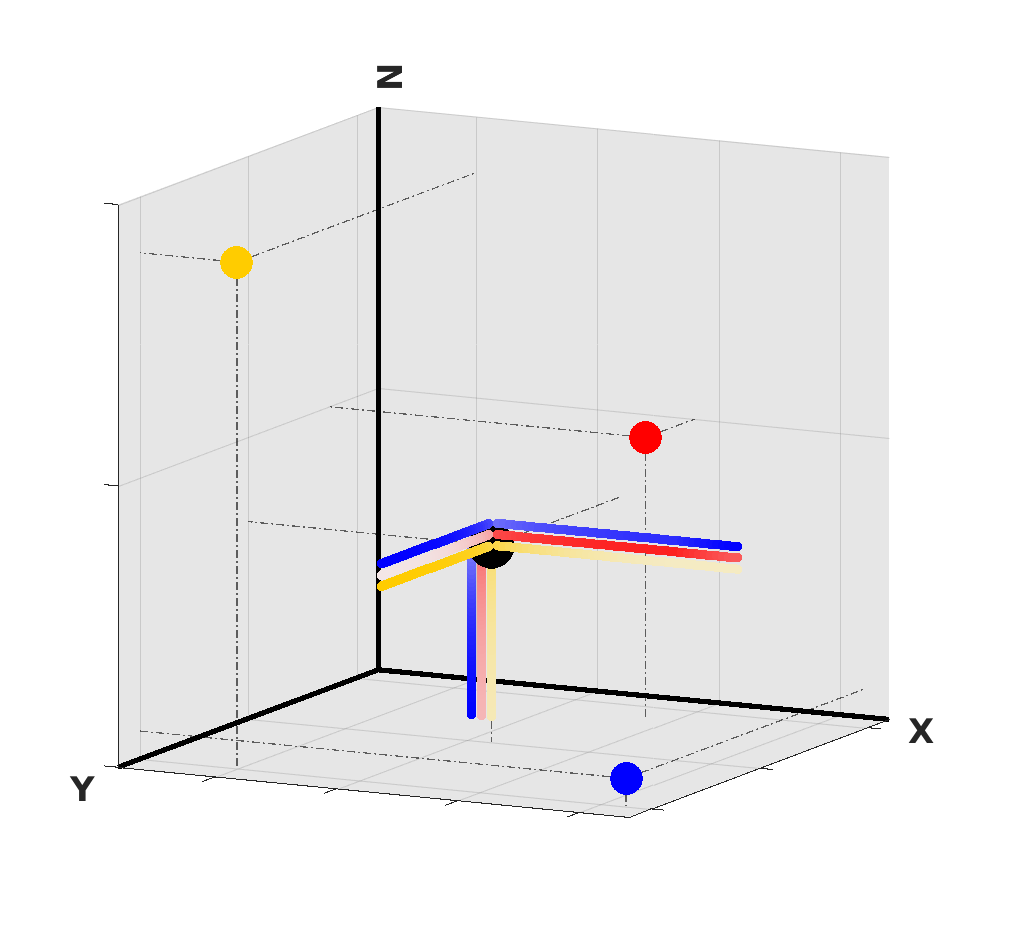
\includegraphics[width = 1\hsize]{Fig3.eps}
	%	\vspace{-0.35cm}
	\caption{Illustration of how goal confidences change upon motion along control dimensions. The three colored lines along each dimension represent the confidences associated with a goal of corresponding color. Brighter and dimmer colors correspond to high and low confidences respectively. One can see that motion along certain control dimensions results in sharper rise in confidences for some goals compared to others, suggesting that the goal disambiguation capabilities are different for different control dimensions.}
	\label{fig:disamb_motivation}
\end{figure}

\subsection{Notation}\label{ssec:notation}
Let $\mathcal{G}$ denote the set of all candidate goals with $n_g = \vert\mathcal{G}\vert$ and let $g^i$ refer to the $i^{th}$ goal with $i \in [1,2,\dots, n_g]$. A \textit{goal} represents the human's underlying intent. Specifically, in assistive robotic manipulation, since the robotic device is primarily used for reaching toward and grasping of discrete objects in the environment, intent inference is the estimation of the probability distribution over all possible discrete goals (objects) in the environment. At any time $t$, the robot actively maintains a probability distribution over goals denoted by $\boldsymbol{p}(t)$ such that $\boldsymbol{p}(t) = [p^1(t), p^2(t),\dots, p^{n_g}(t)]^{T}$ where $p^i(t)$ denotes the probability associated with goal $g^i$.  The probability $p^i(t)$ represent the robot's \textit{confidence} that goal $g^i$ is the human's intended goal. 

Let $\mathcal{K}$ be the set of all controllable dimensions of the robot and $k^i$ represent the $i^{th}$ control dimension where $i \in [1,2,\dots,n_k]$. The cardinality of $\mathcal{K}$ is denoted as $n_k$ and typically depends on the robotic platform used. For example, for a smart wheelchair $n_k = 2$, since the controllable degrees-of-freedom are velocity and heading. Likewise, for a six DoF robotic arm $n_k = 6$, since the controllable degrees-of-freedom correspond to the translation and rotation of the end-effector in the task-space. 

In this work, we assume a kinematic model for the robot and the kinematic state (the robot pose) at any time $t$ is denoted as $\boldsymbol{x}_r(t) \in \mathbb{R}^3 \times \mathbb{S}^3$ and consists of a position component and orientation component.\footnote{$\mathbb{S}^3$ is the space of all unit quaternions.} The pose for goal $g \in \mathcal{G}$ is denoted as $\boldsymbol{x}_g \in \mathbb{R}^3 \times \mathbb{S}^3$. The control command issued by the human via the control interface is denoted as $\boldsymbol{u}_h$ and is mapped to the Cartesian velocity of the robot's end-effector. For a six DoF robotic arm, $\boldsymbol{u}_h \in \mathbb{R}^6$. We also assume the existence of an autonomous robot control policy that generates a robot control command denoted as $\boldsymbol{u}_r \in \mathbb{R}^6$. The control command issued to the robot, which is a synthesis of $\boldsymbol{u}_h$ and $\boldsymbol{u}_r$ (described further in Section~\ref{sec:shared-control}) is denoted by $\boldsymbol{u} \in \mathbb{R}^6$. We also denote the control command that corresponds to a unit velocity vector along the positive and negative directions of control dimension $k$ as $\boldsymbol{e}^k$ and $-\boldsymbol{e}^k$ respectively.

The limitations of the control interfaces necessitate the control space $\mathcal{K}$ to be partitioned into control modes. Let $\mathcal{M}$ denote the set of all control modes with $n_m = \vert\mathcal{M}\vert$. Additionally, let $m^i$ refer to the $i^{th}$ control mode where $i \in [1,2,\dots,n_m]$. Each control mode $m^i$ is a subset of $\mathcal{K}$ such that $\bigcup\limits_{i=1}^{n_m} m^i$ spans all of the controllable dimensions. A dimension $k \in \mathcal{K}$ can be an element of multiple control modes.

%\deleted{Let $\boldsymbol{e}^i$ be the standard basis vectors that denote the unit velocity vector along the $i^{th}$ control dimension. For the rotational control dimensions, the velocity is specified with respect to the end-effector of the robotic frame. (used to be footnote). The robot pose and the goal pose for $g \in \mathcal{G}$ are denoted $\boldsymbol{x}_r$ and $\boldsymbol{x}_g$ respectively and $\boldsymbol{u}_h$ denotes the human control command.}

\subsection{Disambiguation Metric}\label{ssec:disamb}
The disambiguation metric that we develop in this paper is a heuristic measure that characterizes the intent disambiguation capabilities of a control dimension $k \in \mathcal{K}$ and is denoted by $D_k \in \mathbb{R}$. We explicitly define disambiguation metrics for both positive negative motions along $k$ as $D_k^{+}$ and $D_k^{-}$ respectively. We also define a disambiguation metric $D_m \in \mathbb{R}$ for each control mode $m \in \mathcal{M}$.

The disambiguation metric $D_m$ is a measure of how useful the user control commands would be \textit{for} the robot to perform more accurate intent inference if the user were to operate the robot in control mode $m$. Both $D_k$ and $D_m$ will be formally defined in Section~\ref{ssec:components}.
The computation of $D_k$ depends on four features (denoted as $\Gamma_k$, $\Omega_k$, $\Lambda_k$ and $\Upsilon_k$), that capture different aspects of the shape of a projection of the probability distribution over intent. These projections and computations are described in detail in Section~\ref{ssec:projection} and Section~\ref{ssec:components}, and as a pseudocode in Algorithm~\ref{alg1}. The disambiguation formalism developed in this section is agnostic to the particular form of intent inference. However, the algorithm assumes that $\boldsymbol{p}(t)$ can be forward projected in time by iteratively applying the intent inference algorithm. 


\subsection{Forward Projection of $\boldsymbol{p}(t)$}\label{ssec:projection}
The first step towards the computation of $D_k$ is the forward projection of the probability distribution $\boldsymbol{p}(t)$ from the current time $t_a$ to $t_b$ and $t_c$ ($t_a < t_b < t_c$), Algorithm~\ref{alg1}, lines 3-13. We consider two projection times ($t_b$ and $t_c$) in order to compute short-term and long-term behavior and evolution of the probability distribution. Application of control command $\boldsymbol{e}^k$ results in probability distributions $\boldsymbol{p}^+_k(t_b)$, $\boldsymbol{p}^+_k(t_c)$ and $-\boldsymbol{e}^k$ results in $\boldsymbol{p}^-_k(t_b)$ and $\boldsymbol{p}^-_k(t_c)$, where the subscript $k$ denotes the fact that the projection is the result of the application of a control command only along control dimension $k$. Note that Algorithm~\ref{alg1} is run twice to compute the projected probability distributions for $\boldsymbol{e}^k$ and $-\boldsymbol{e}^k$. All parameters and features which affect the computation of $\boldsymbol{p}(t)$ are denoted as $\boldsymbol{\Theta}$. 

\begin{algorithm}[t]
	\caption{Intent Disambiguation}
	\label{alg1}
	\begin{algorithmic}[1]
		\REQUIRE $\boldsymbol{p}(t_a), \boldsymbol{x}_r(t_a), \Delta t, t_a < t_b < t_c, \boldsymbol{\Theta}$
		\FOR{$k=0\dots n_k$}
		\STATE Initialize $D_k = 0$, $t = t_a$

		\WHILE{$t \leq t_c$}
			\STATE $\boldsymbol{p}_k(t + \Delta t) \leftarrow \text{UpdateIntent}(\boldsymbol{p}_k(t), \boldsymbol{u}_h; \boldsymbol{\Theta})$
			\STATE $\boldsymbol{x}_r(t + \Delta t) \leftarrow \text{SimulateKinematics}(\boldsymbol{x}_r(t), \boldsymbol{u}_h)$
			\IF{$t = t_b$} \STATE {$Compute \;\;\Gamma_k, \Omega_k, \Lambda_k$} 
			\ENDIF
			\IF{$t = t_c$} \STATE{$Compute \;\;\Upsilon_k$} \ENDIF
			\STATE $t \leftarrow t + \Delta t$
		\ENDWHILE

		\STATE $Compute \;\;D_k$
		\ENDFOR
		
	\end{algorithmic}
\end{algorithm}

\subsection{Features of $D_k$}\label{ssec:components}
\begin{figure*}[t]
	\centering
	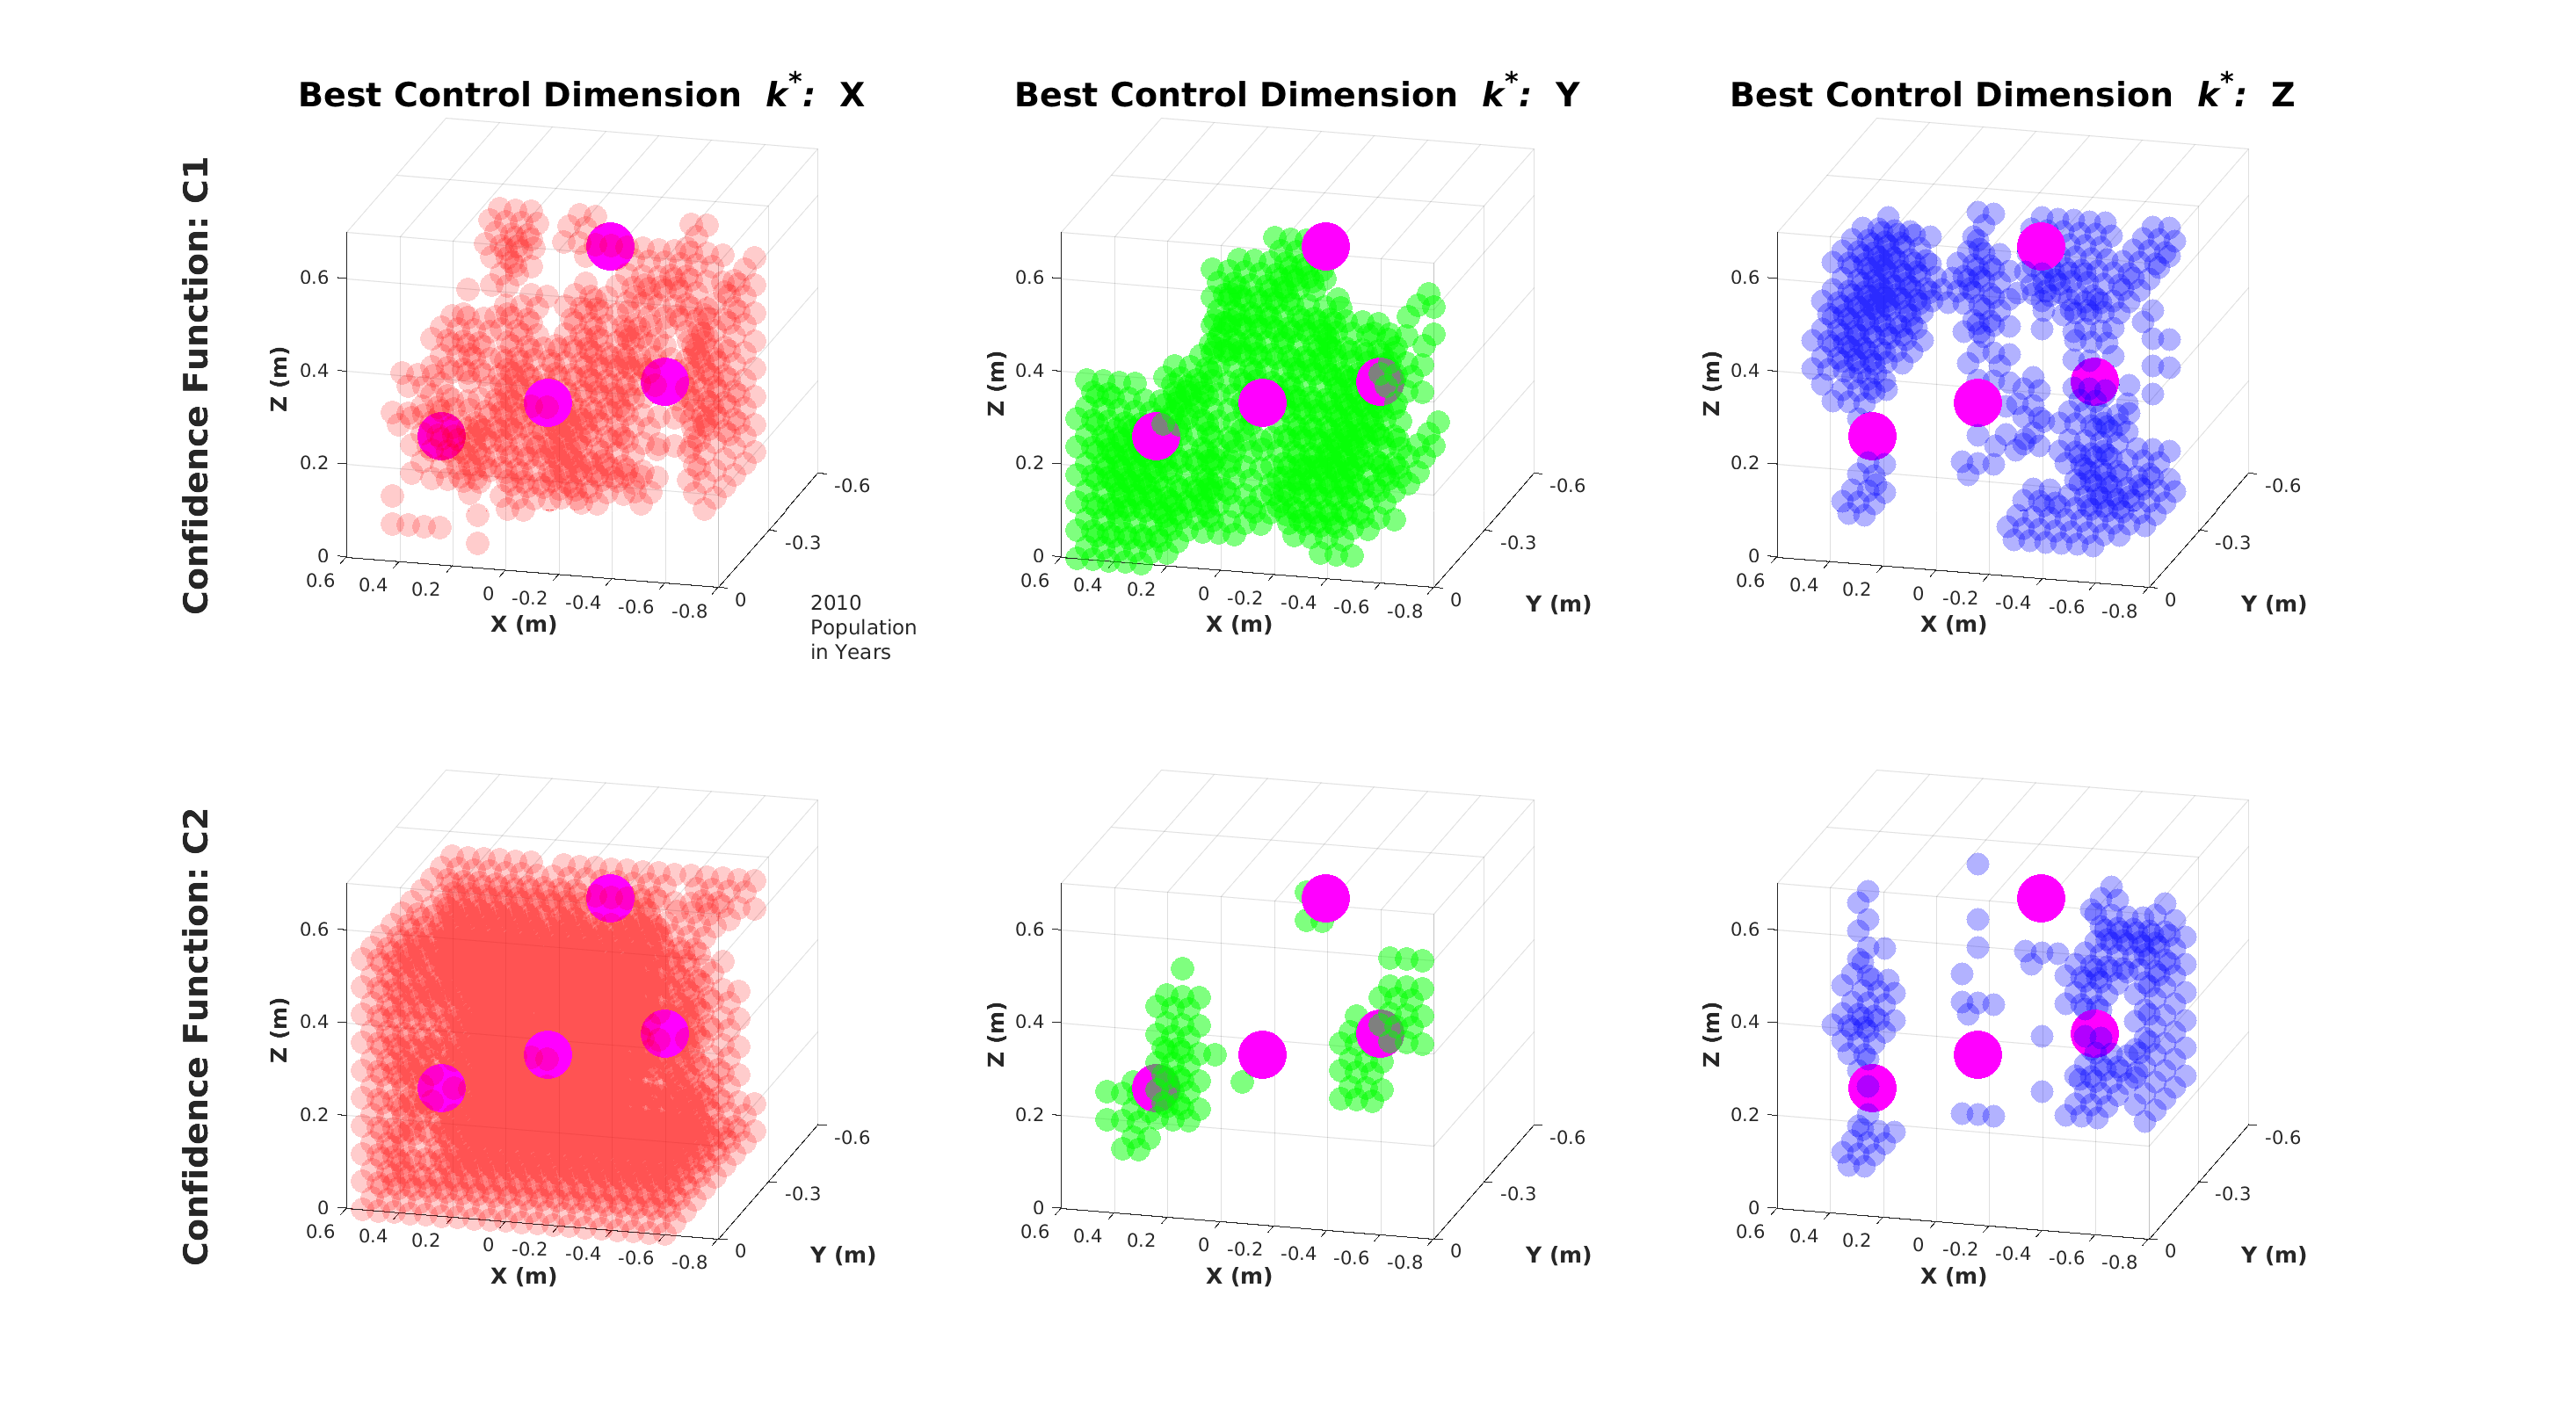
\includegraphics[width = 1.15\hsize, height = 0.6\vsize, center]{Fig4.eps}
	\caption{Control dimensions best able to disambiguate intent.  Left column: $k^*$ is X. Middle Column: $k^*$ is Y. Right Column: $k^*$ is Z. Magenta spheres indicate the goal locations (intent). In this example, the goals are spread maximally along the $x$ and $z$ dimensions, and so inference happens more quickly if the human control commands are along $x$ or $z$. We see that $x$ and $z$ are chosen more often as the most disambiguating dimensions when using intent inference function C2 (bottom row). Function C2 considers the instantaneous directedness of the human's control command towards that goal, while inference function C1 (top row) encodes only proximity to a given goal. Function C2 is considered to encode more information about the human's intent than C1, with the result of stronger inference power---which is inherently linked to the disambiguation power of our algorithm. Further details in~\citep{gopinath2017mode}.}
	\label{fig:sim_res}
\end{figure*}
Informed by our initial empirical investigations, we hand-design four features that encode different aspects of the shape of the probability distribution as it evolves under user control in a specific control dimension $k$. For each control dimension $k$, each of the four features is computed for projections along both positive and negative directions independently. The four features are computed in lines 7 and 10 in Algorithm~\ref{alg1}.

1) \textit{Maximum probability:} The maximum of the projected probability distribution $\boldsymbol{p}_k(t_b)$ is a good measure of the robot's \textit{overall certainty} in accurate predicting human intent (The maximum of this discrete probability distribution is the mode of the distribution). We define the distribution maximum as $\Gamma_k$.
\begin{equation}
\Gamma_k = \max\limits_{1 \leq i \leq n_g}p^i_k(t_b)
\end{equation}
A higher value implies that the robot has a greater confidence in its prediction of the human's intended goal.

2) \textit{Difference between largest probabilities:} Disambiguation accuracy benefits from greater differences between the first and second most probable goals. This difference is denoted as $\Omega_k$.
\begin{equation}
\Omega_k = \text{max}(\boldsymbol{p}_k(t_b)) - \text{max}(\boldsymbol{p}_k(t_b) \setminus \text{max}(\boldsymbol{p}_k(t_b)))
\end{equation}
$\Omega_k$ becomes important in situations in which the distribution can have multiple modes and a measure of overall certainty ($\Gamma_k$) alone is not sufficient for successful disambiguation. 

3) \textit{Pairwise separation of probabilities:} If the difference between the largest probabilities fails to disambiguate, then the separation, $\Lambda_k$, in the remaining goal probabilities will further aid in intent disambiguation. The quantity $\Lambda_k$ is computed as the \textit{sum of the pairwise distances} between the $n_g$ probabilities.
\begin{equation}
\Lambda_k = \sum_{i=1}^{n_g}\sum_{j=i}^{n_g}\lvert p^i_k(t_b) - p^j_k(t_b)\rvert
\end{equation}

4) \textit{Gradients:} $\Gamma_k, \Omega_k$ and $\Lambda_k$ are local measures that encode shape characteristics of the short-term temporal projections of the probability distribution over goals. However, the quantity $\boldsymbol{p}_k(t)$ can undergo significant changes upon long-term continuation of motion along control dimension $k$. The spatial gradient of $\boldsymbol{p}_k(t)$ encodes this propensity for change and is approximated by 
\begin{equation*}
\frac{\partial\boldsymbol{p}_k(t)}{\partial x_k} \simeq \frac{\boldsymbol{p}_k(t_c) - \boldsymbol{p}_k(t_b)}{x_k(t_c) - x_k(t_b)}
\end{equation*}
where $x_k$ is the component of robot's projected displacement along control dimension $k$. The greater the difference between individual spatial gradients, the greater will the probabilities deviate from each other, thereby helping in disambiguation. In order to quantify the ``spread'' of gradients we define a quantity $\Upsilon_k$ 
\begin{equation}
\Upsilon_k = \sum_{i=1}^{n_g}\sum_{j=i}^{n_g}\Big \lvert\frac{\partial p^i_k(t)}{\partial x_k} - \frac{\partial p^j_k(t)}{\partial x_k}\Big \rvert
\end{equation}
where $\lvert\cdot\rvert$ denotes the absolute value. 

5) \textit{Putting it all together:} 
The individual features $\Gamma_k$, $\Omega_k$, $\Lambda_k$ and $\Upsilon_k$ are then combined to compute $D_{k}$ in such a way that, by design, higher values of $D_k$ imply greater disambiguation capability for the control dimension $k$. More specifically, $D_k$ is denoted as 
\begin{equation}\label{DK}
D_{k} = \underbrace{w\cdot(\Gamma_k\cdot \Omega_k\cdot\Lambda_k)}_{\text{short-term}} + \underbrace{(1 - w)\cdot \Upsilon_k}_{\text{long-term}}
\end{equation}
where $w$ is a task-specific weight that balances the contributions of the short-term and long-term components. (In our implementation, $w$ was set at $0.5$ empirically.) Equation~\ref{DK} actually is computed twice, once in each of the positive ($\boldsymbol{e}^k$) and negative directions ($-\boldsymbol{e}^k$) along $k$, and the results ($D_k^+$ and $D_k^-$) are then summed. 

The computation of $D_k$ is performed for each control dimension $k \in \mathcal{K}$. The disambiguation metric $D_m$ for control mode $m$ then is calculated as 
\begin{equation*}\label{EQ2}
D_m = \sum_{k} D_{k} \;
\end{equation*}
where $k \in m$ iterates through the set of control dimensions on which $m$ is able to operate.
The control mode with highest disambiguation capability $m^*$ is given by
\begin{equation*}
m^* = \argmax_m  D_{m}
\end{equation*}
while $k^* = \argmax_k D_k$ gives the control dimension with highest disambiguation capability $k^{*}$.
%\begin{equation*}
%k^* = \argmax_k D_k~~~.
%\end{equation*}
Disambiguation mode $m^{*}$ is the mode that the algorithm chooses \textit{for} the human to better estimate their intent. 

\section{Intent Inference}\label{sec:inference}
This section describes the intent inference scheme used in this paper. Our preliminary work~\citep{gopinath2017mode} revealed that the power of our disambiguation algorithm proposed in Section~\ref{ssec:disamb} is intimately linked with the inference power of different choices of intent inference mechanisms. In this work, we propose a novel intent inference scheme inspired by \textit{dynamic field theory}. We detail this approach in Section~\ref{ssec:ii_dft} and provide in Section~\ref{ssec:baseline} a qualitative baseline comparison to an inference formulation from shared-control literature. 

\subsection{Intent inference based on Dynamic Field Theory}\label{ssec:ii_dft}
Our novel intent inference approach is inspired by \textit{dynamic field theory}, in which the time evolution of the probability distribution $\boldsymbol{p}(t)$ is specified as a dynamical system with constraints. Unlike Bayesian approaches used in shared-control teleoperation systems, our approach does not assume continuous user input~\citep{dragan2013policy,pellegrinelli2016human}; this is important especially in the domain of assistive robotics in which user input is typically intermittent due to inherent motor or cognitive limitations. By casting the time-evolution of the distribution as a dynamical system, information from the past states can be easily incorporated (for example, via a low-pass filter that smooths the evolution). Furthermore, Bayesian approaches require a model for how the user operates the robot (the likelihood function) and typically user policy is modeled assuming that the user optimizes a cost function according to the maximum entropy principle~\citep{javdani2017shared, ziebart2008maximum}. Our intent inference approach does not require any such assumptions and allows for suboptimal human performance. The critical piece in the dynamical system is a `forcing function' that drives the evolution of the distribution to different states, the design of which is informed by what features of the human input capture the underlying human intent most effectively. 

 Section~\ref{sssec:dft} provides a primer on the basic principles and features of \textit{dynamic field theory} and its application in the fields of neuroscience and cognitive robotics. Section~\ref{sssec:dft_ii} describes our novel formulation that makes use of dynamic field theory for the purposes of intent inference. 

\subsubsection{Dynamic Field Theory}\label{sssec:dft}

In Dynamic Field Theory (DFT)~\citep{schoner2015dynamic}, variables of interest are treated as dynamical state variables. To represent the information about these variables requires two dimensions: one which specifies the value the variables can attain (the domain) and the other which encodes the \textit{activation level} or the amount of information about a particular value. These \textit{activation fields} are analogous to probability distributions defined over a random variable. 

Following Amari's formulation~\citep{amari1977dynamics} dynamics of an activation field $\phi(x, t)$ are given by 
\begin{multline*}
\tau\dot{\phi}(x,t) = -\phi(x,t) + h + S(x,t) + \\ \int\limits_{}^{}dx^{\prime}b(x-x^{\prime})\sigma(\phi(x^{\prime}, t)) 
\end{multline*} 
where $x$ denotes the variable of interest, $t$ is time, $\tau$ is the time-scale parameter, $h$ is the constant resting level, and $S(x,t)$ is the external input, $b(x-x^\prime)$ is the interaction kernel and $\sigma(\phi)$ is a sigmoidal nonlinear threshold function. The interaction kernel mediates how activations at all other field sites $x^\prime$ drive the activation level at $x$. Two types of interactions are possible: excitatory (when interaction is positive) which drives up the activation, and inhibitory (when the interaction is negative) which drives the activation down. 
%\deleted{Historically, dynamic neural fields originally were conceived to explain cortical population neuronal dynamics, based on the hypothesis that the excitatory and inhibitory neural interactions between local neuronal pools form the basis of cortical information processing}~\citep{wilson1973mathematical}. 

Dynamic neural fields possess some unique characteristics that make them ideal candidates for modeling higher-level cognition. First, a peak in the activation field can be \textit{sustained} even in the absence of external input due to the recurrent interaction terms. Second, information from the past can be \textit{preserved} over much larger time scales quite easily by tuning the time-scale parameter thereby endowing the fields with memory. Third, the activation fields are \textit{robust} to disturbance and noise in the external output~\citep{schoner2008dynamical}. 
As a result, DFT principles have found widespread application in the area of cognitive robotics~\citep{erlhagen2006dynamic}, specifically in the contexts of efficient human-robot interaction~\citep{erlhagen2014dynamic}, robotic scene representation~\citep{zibner2011dynamic}, obstacle avoidance and target reaching behaviors in both humans and robots~\citep{schoner1995dynamics}, and for object learning and recognition~\citep{faubel2008learning}. 


\subsubsection{Dynamic Neural Fields for Intent Inference}\label{sssec:dft_ii}

Recurrent interaction between the state variables, 
robustness to noise and inherent memory make dynamic neural fields an ideal candidate for intent inference. 

Our insight is to use the framework of dynamic neural fields to specify the time evolution of the probability distribution $\boldsymbol{p}(t)$, in which we treat the individual goal probabilities $p^i(t)$ as constrained dynamical state variables such that $p^i(t) \in [0, 1]$ and $\Sigma_{1}^{n_g}p^{i}(t) = 1$. The dynamical system can be generically written as 
\begin{equation*}
\dot{\boldsymbol{p}}(t) = F(\boldsymbol{p}(t), \boldsymbol{u}_h ; \boldsymbol{\Theta})
\end{equation*}
where $F$ represents a nonlinear vector field, $\boldsymbol{u}_h$ is the human control input and $\boldsymbol{\Theta}$ represents all other task-relevant features and parameters that affect the time-evolution of the probability distribution. 
The full specification of the neural field is given by
\begin{multline}\label{eq:dft}
\frac{\partial \boldsymbol{p}(t)}{\partial t} = \frac{1}{\tau}\bigg[-\mathbb{I}_{n_g\times n_g}\cdot\boldsymbol{p}(t) + \underbrace{\frac{1}{n_g}\cdot\mathbbm{1}_{n_g}\bigg]}_{\text{rest state}} + \\ \underbrace{\boldsymbol{\lambda}_{n_g\times n_g}\cdot\sigma(\boldsymbol{\xi}(\boldsymbol{u}_h;\boldsymbol{\Theta}))}_{\text{excitatory + inhibitory}}
\end{multline}
where time-scale parameter $\tau$ determines the memory capacity of the system, $\mathbb{I}_{n_g\times n_g}$ is the identity matrix, $\mathbbm{1}_{n_g}$ is a vector containing all ones of dimension $n_g$, $\boldsymbol{\lambda}$ is the control matrix that controls the excitatory and inhibitory aspects, $\boldsymbol{\xi}$ is a function that encodes the nonlinearity through which human control commands and task features affect the time evolution, and $\sigma$ is a biased sigmoidal nonlinearity given by $\sigma(\boldsymbol{\xi}) = \frac{1}{1 + e^{-\boldsymbol{\xi}}} - 0.5$.
%The off-diagonal elements of $\boldsymbol{\lambda}$ mediate the interaction between all of the probabilities. In the absence of any information or cues, the probability distribution settles to a resting state which is a uniform distribution, this is  because $\boldsymbol{u}_h = 0$, $\boldsymbol{\xi} = \vec{0}$. \deleted{That is, in the absence of any human control command, the probability distribution decays to the resting state which is a uniform distribution. }

The design of $\boldsymbol{\xi}$ is informed by what features of the human control input and environment capture the human's underlying intent most effectively. For example, motion cues reveal a great deal about the underlying intention and have been successfully used in different intent inference schemes~\citep{barrett2005accurate}. We rely on the \textit{directedness} of the robot motion towards a goal, the \textit{agreement} between the human commands and robot autonomy and the \textit{proximity} to a goal. 
With $\boldsymbol{\Theta} = \{\boldsymbol{x}_r, \boldsymbol{x}_{g^i}, \boldsymbol{u}_{r, g^i}\}$, one dimension $i$ of $\boldsymbol{\xi}$ is defined as 
\begin{multline*}
\xi^i(\boldsymbol{u}_h;\boldsymbol{x}_r, \boldsymbol{x}_{g^i}, \boldsymbol{u}_{r, g^i}) = \underbrace{\frac{1 + \eta}{2}}_{\text{directedness}} + \underbrace{\boldsymbol{u}_{h}^{rot}\cdot\boldsymbol{u}_{r,g^i}^{rot}}_{\text{agreement}}
\\+ \underbrace{\text{max}\Big(0, 1-\frac{\norm{\boldsymbol{x}_{g^i} - \boldsymbol{x}_r}}{R}\Big)}_{\text{proximity}}
\end{multline*}
where  $\eta = \frac{\boldsymbol{u}_h^{trans}\cdot(\boldsymbol{x}_{g^i} - \boldsymbol{x}_r)^{trans}}{\norm{\boldsymbol{u}_h^{trans}}\norm{(\boldsymbol{x}_{g^i} - \boldsymbol{x}_r)^{trans}}}$, $\boldsymbol{u}_{r,g^i}$ is the robot autonomy command for reaching goal $g^i$, $trans$ and $rot$ refer to the translational and rotational components of a command $\boldsymbol{u}$ or position $\boldsymbol{x}$,  $R$ is the radius of the sphere beyond which the proximity component is always zero, and $\norm{\cdot}$ is the Euclidean norm. The \textit{directedness} component captures the likelihood of a user taking the shortest straight line path towards a goal $g$ (equivalent to a user optimizing a straight line distance based cost function), whereas the \textit{agreement} measures the alignment of the human's input to the autonomy command in the end-effector's rotation space and serves as an indicator of the how the human cooperates with autonomy.

Given the initial probability distribution at time $t_a$ Equation~\ref{eq:dft} can be solved numerically from $t \in [t_a, t_b]$ using a simple Euler algorithm with a fixed time-step $\Delta t$. At every time-step the constraints on $p^i(t)$ are enforced thereby ensuring that $\boldsymbol{p}(t)$ is a valid probability distribution. 
The most confident goal $g^*$ is computed as $g^* = \argmax_i  p^i(t)$.


\subsection{Baseline Comparison}\label{ssec:baseline}
In this section we provide a qualitative baseline comparison of our proposed intent inference method against a Bayesian inference scheme that is used in shared autonomy in teleoperation~\citep{dragan2012assistive,admoni2016predicting, javdani2017shared}. Under the Bayesian approach, the user is typically modeled as a Markov Decision Process and is assumed to noisily optimize a cost function according to the maximum entropy principle~\citep{ziebart2008maximum}. 

\begin{figure}[t]
	\centering
	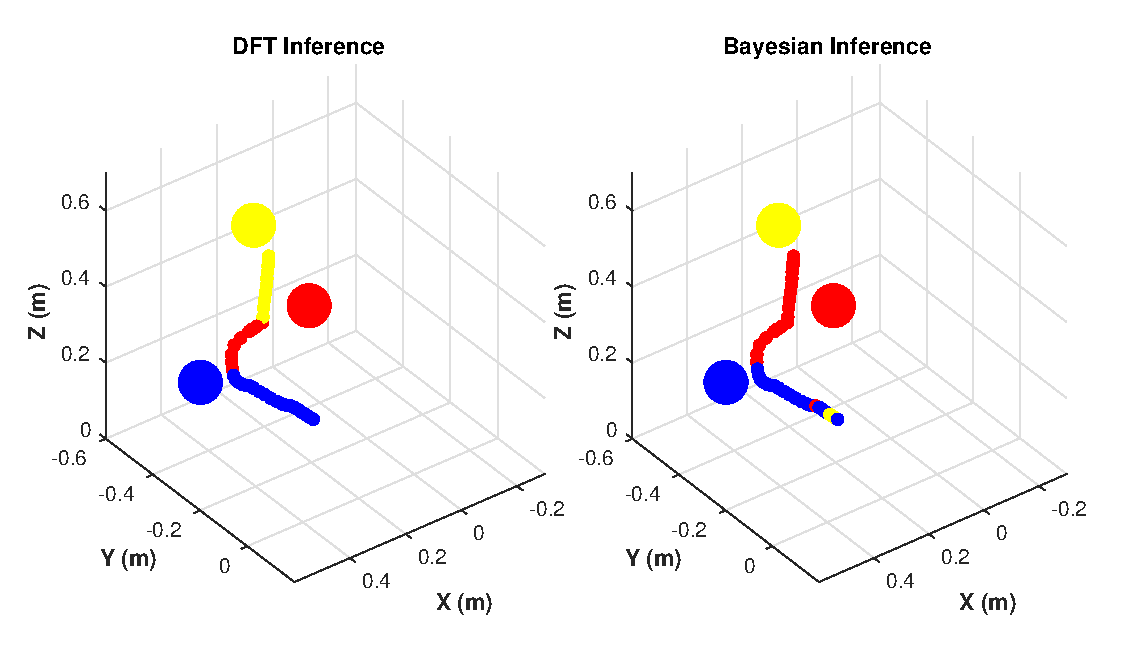
\includegraphics[width = 1\hsize, height = 0.18\vsize]{Fig5.eps}
	%	\vspace{-0.35cm}
	\caption{Goal inference using our dynamic field theory (DFT) approach (left) and the Bayesian approach~\cite{dragan2013policy} (right). Goals shown as circles. The motion trajectory is colored according to the goal prediction made at that location during the execution. The human operator first reaches towards the blue goal, then the red and finally the yellow.}
	\label{fig:intent_comp}
\end{figure}
Figure~\ref{fig:intent_comp} shows an illustrative comparison of goal inference using our dynamic field theory based approach and the Bayesian approach using a distance based cost function.

In this example, the user's intended goal changes during the execution: first reaching towards the blue goal, then switching to the red and finally settling on the yellow goal. We can see that the two inference approaches are comparable for the first two segments of the trajectory. For the final segment, the Bayesian inference method was unable to produce the correct inference due to the posterior distribution  collapsing to a delta function. However, the dynamic neural field based approach was successful in producing the correct inference at all times. The posterior collapse to a delta function in Bayesian inference is primarily due to numerical errors and can be avoided by adding some amount of noise to the prior at every time-step, however then this becomes yet another heuristic for practical success. In general, both inference approaches consistently produce similar performances for a wide variety of goal configurations. For goal poses that include orientation information, the Bayesian approach will work only if the cost function also depended on the `distance' traversed in the orientation space. The inference accuracy is highly dependent on the choice of the user model (the likelihood function) for Bayesian schemes and on $\boldsymbol{\xi}$ for DFT based approach. 

Here we emphasize a few fundamental differences between the Bayesian scheme and the dynamical field theory based approach. First, the DFT approach does not assume continuous input from the user and in the absence of user input the in-built `forgetting' mechanism causes the distribution to gradually settle down to a uniform distribution. Secondly, unlike the Bayesian approach the DFT approach does not rely on an explicit user model and therefore can handle suboptimal user input seamlessly. Third, the Bayesian approach is made tractable using a Laplacian approximation of the cost function around an optimal trajectory; however for trajectories that deviate a great deal from the optimal trajectory the second-order approximation is less accurate. \added{Note: this is just a mathematical fact, based on the derivation presented in the Dragan's paper. I am finding it hard to tie it to the example shown here} 
%
%Dragan et al assumes continuous input. This is not necesarily the case in assistive robotics in which users swithc modes or have limited capability to provide continuous input. Laplacian approximation is not necessarily valid when the trajectory is FAR from optimal! Cost function is quadratic. Heurstic cost functions for high dimensional problems such as manipulation. }

	
\section{Shared Control}\label{sec:shared-control}
The shared-control paradigm implemented on our robot is a blending-based approach in  which the final control command issued to the robot is a linear composition of the human control command and an autonomous robot policy.
The autonomous control policy generates control command
$\boldsymbol{u}_r \leftarrow f_{a}(\boldsymbol{x}_r)$
where $f_{a}(\cdot) \in \mathcal{F}_{a}$, and $\mathcal{F}_{a}$ is the set of all control behaviors corresponding to different tasks. This set could be derived using a variety of techniques such as \textit{Learning from Demonstrations}~\citep{argall2009survey, schaal1997learning}, motion planners~\citep{hsu2002randomized,ratliff2009chomp} or navigation functions~\citep{rimon1992exact,tanner2003nonholonomic}. Specifically, let $\boldsymbol{u}_{r,g}$ be the autonomy command associated with goal $g$. The final control command $\boldsymbol{u}$ issued to the robot then is given by
\begin{equation*}
\boldsymbol{u} = \alpha\cdot \boldsymbol{u}_{r,g^*} + (1 - \alpha)\cdot \boldsymbol{u}_h
\end{equation*}
where $g^*$ is the most confident goal. Similar to $\boldsymbol{u}_h$, the autonomy command $\boldsymbol{u}_{r, g^*}$ is mapped to the 6D Cartesian velocity of the end-effector, $\boldsymbol{u}_{r, g^*} \in \mathbb{R}^6$. The robot state evolves according to the kinematic equation given by,
\begin{equation*}
\boldsymbol{x}_r(t+\Delta t) = f_{kin}(\boldsymbol{x}_r(t), \boldsymbol{u}(t))
\end{equation*}
where, $f_{kin}(\cdot)$, denotes the nonlinear kinematics of the robot and $\Delta t$ is the Euler time-step.
  The blending factor $\alpha$ is a piecewise linear function of the probability $p(g^*)$ associated with $g^*$ and is given by
$$
\alpha = \left\{
\begin{array}{ll}
0 & \quad\quad~~~ p(g^*) \leq \rho_1 \\
\frac{\rho_3 (p(g^*) - \rho_1)}{\rho_2 - \rho_1}  &  \quad \text{if}\quad \rho_1 < p(g^*) \leq \rho_2  \\
\rho_3 & \quad\quad~~~ p(g^*) > \rho_2 	
\end{array}
\right.
$$
with $\rho_i \in [0, 1] \;\forall\; i \in [1,2,3]$ and $ \rho_2 > \rho_1$. 
In our implementation, we empirically set $\rho_1 = \frac{1.2}{n_g}, \rho_2 = \frac{1.4}{n_g}$ and $ \rho_3 = 0.7$.

The robot control command $\boldsymbol{u}_{r,g}$ is generated using a simple potential field which is defined in all parts of the state space~\citep{khatib1986real}. Every goal $g$ is associated with a potential field $\gamma_g$ which treats $g$ as an attractor and all the other goals in the scene as repellers. For potential field $\gamma_g$, the attractor velocity is given by
\begin{equation*}
\dot{\boldsymbol{x}}_r^{attract} = \boldsymbol{x}_{g} - \boldsymbol{x}_r
\end{equation*}
where $\boldsymbol{x}_{g}$ is the location of goal $g$.\footnote{In position space, the `--' operator computes the difference between the goal position and current robot position in $\mathbb{R}^3$. In orientation space, the `--' operator computes the \textit{quaternion difference} between the goal orientation and the current robot orientation.} The repeller velocity is given by
\begin{equation*}
\dot{\boldsymbol{x}}_r^{repel} = \sum_{i \in \mathcal{G} \setminus g} \frac{\boldsymbol{x}_r - \boldsymbol{x}_{g^i}}{\mu(\norm{\boldsymbol{x}_r - \boldsymbol{x}_{g^i}}^2)}
\end{equation*}
where $\dot{\boldsymbol{x}}_r$ indicates the velocity of the robot in the world frame, $\mu$ controls the magnitude of the repeller velocity and $\norm{\cdot}$ is the Euclidean norm. The autonomy command is computed as a summation of these attractor and repeller velocities.
\begin{equation*}
\boldsymbol{u}_{r,g} = \dot{\boldsymbol{x}}_r^{attract} + \dot{\boldsymbol{x}}_r^{repel} 
\end{equation*}
$\gamma_g$ operates in the full six dimensional Cartesian space, and treats position and orientation as independent potential fields. 


\begin{figure*}[ht!]
	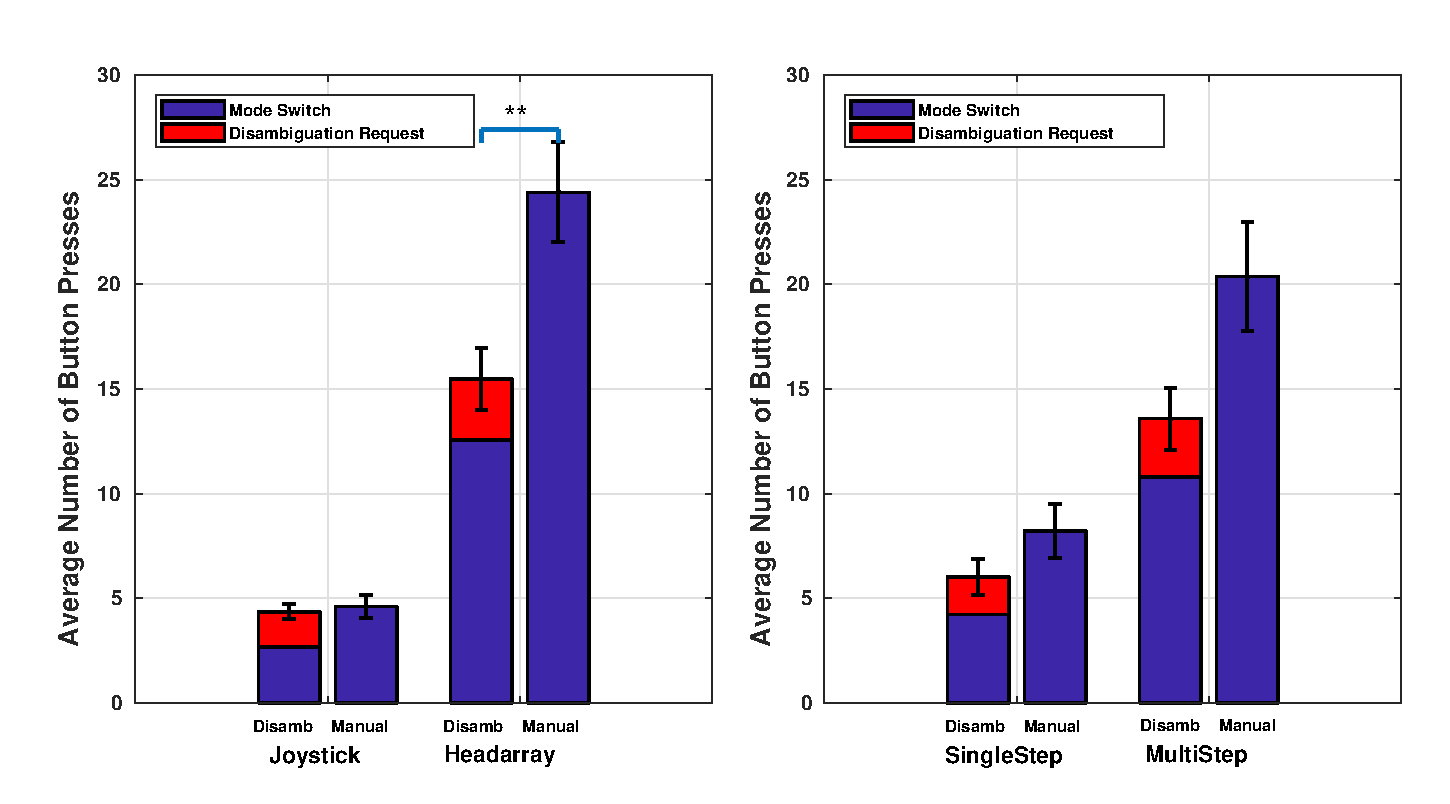
\includegraphics[keepaspectratio, width = \textwidth ]{Fig7.eps}
	\caption{Study tasks performed by subjects. \textit{Left:} Single-step reaching task. \textit{Right:} Multi-step Pouring task. }
	\label{fig:tasks}
\end{figure*}

\section{Study Methods}\label{sec:ed}
In this section, we describe the study methods used to evaluate the efficacy of the disambiguation system. 
\subsection{Participants}
For this study eight subjects were recruited (mean age: $31 \pm 11$, 3 males and 5 females). All participants gave their informed, signed consent to participate in the experiment, which was approved by Northwestern University's Institutional Review Board.
\subsection{Hardware}\label{ssec:hardware}
The experiments were performed using the MICO 6-DoF robotic arm (Kinova Robotics, Canada), specifically designed for assistive purposes. The software system was implemented using the Robot Operating System (ROS) and data analysis was performed in MATLAB. 

The subjects teleoperated the robot using two different control interfaces: a 2-axis joystick and a switch-based head array. The control signals captured from the interfaces were mapped to the Cartesian velocities of the end-effector (Figure~\ref{fig:interfaces}).
\begin{figure}[b]
	\centering
	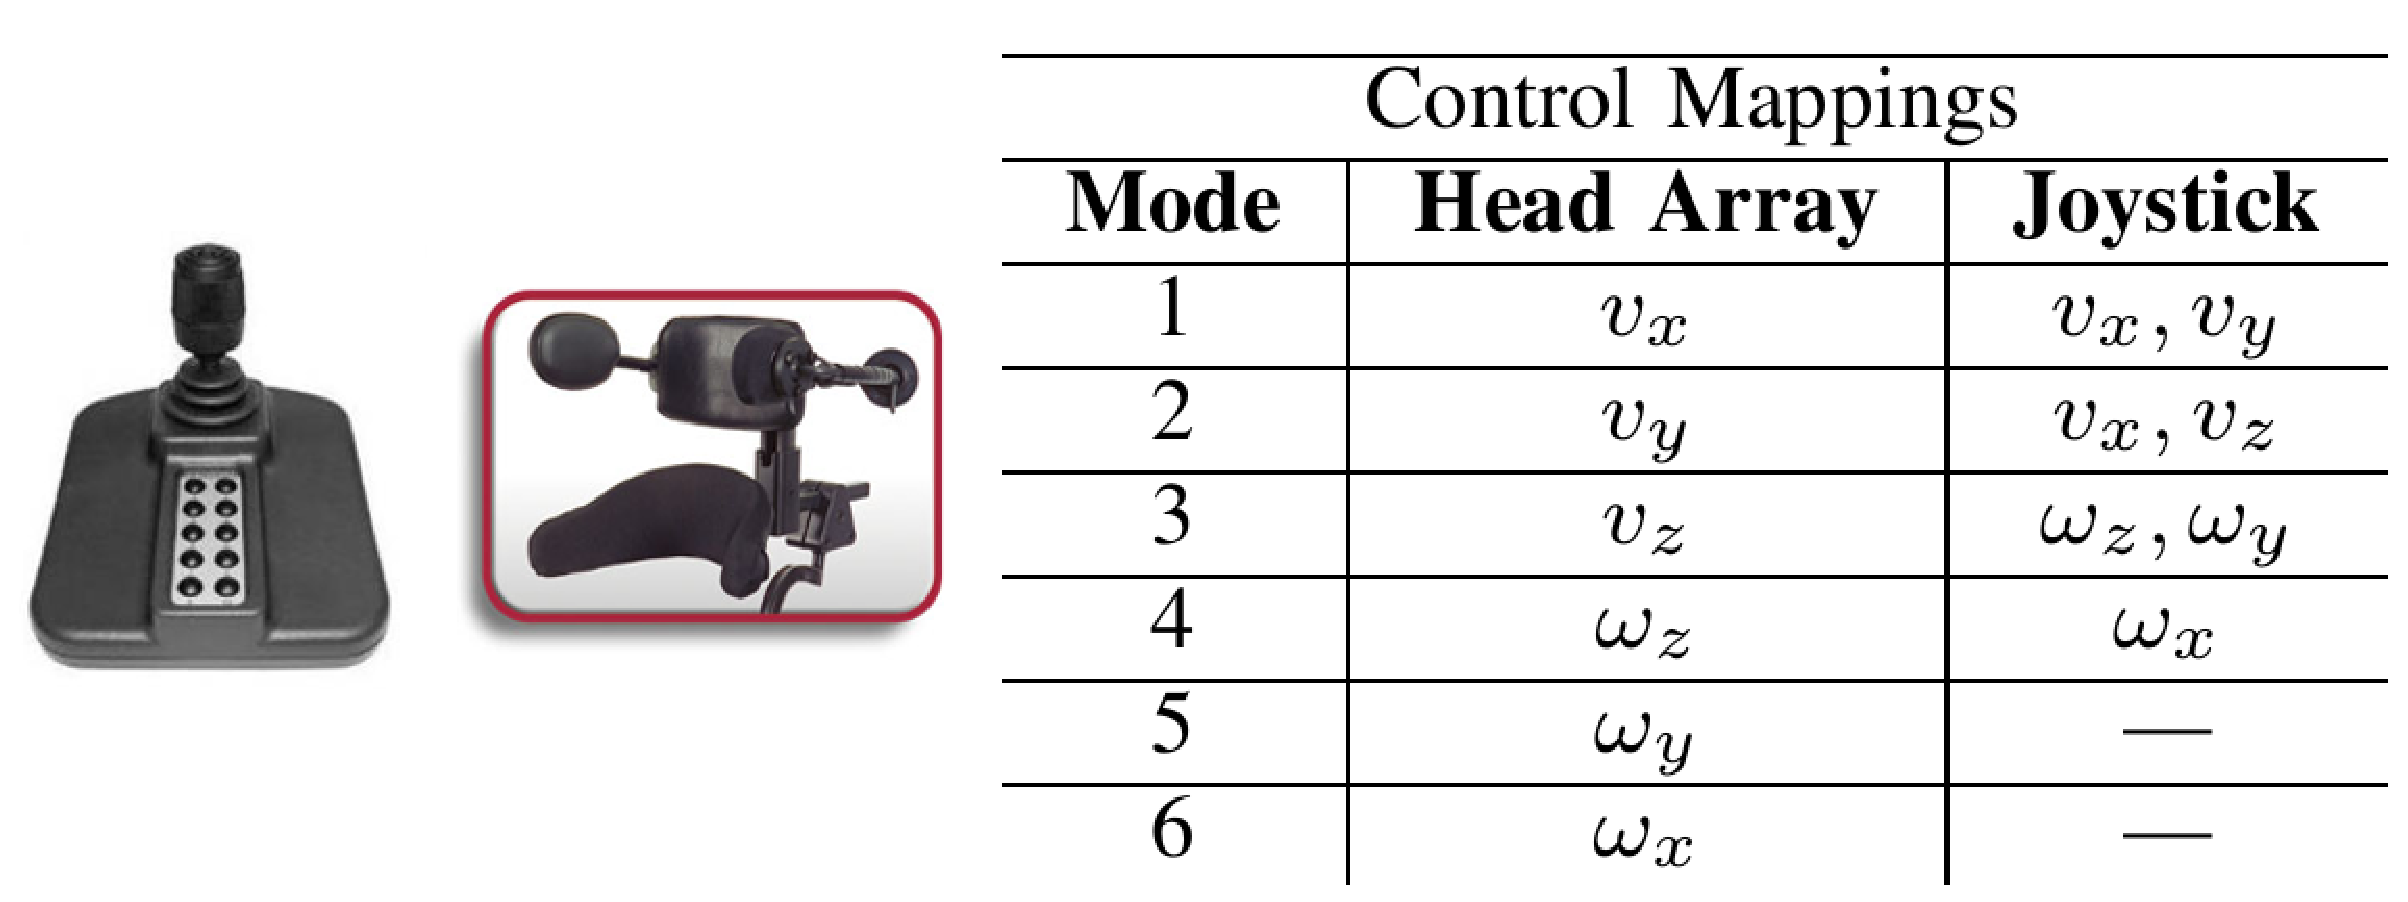
\includegraphics[width = 1\hsize, height = 0.13\vsize]{Fig6.eps}
	%	\vspace{-0.35cm}
	\caption{A 2-axis joystick (left) and switch-based head array (center) and their operational paradigms (right). $v$ and $\omega$ indicate the translational and rotational velocities of the end-effector, respectively.}
	\label{fig:interfaces}
\end{figure}

The joystick generated continuous control signals and allowed for control of a maximum of two dimensions at a time. The 6-D control space was partitioned into four control modes that could be accessed using the buttons on the joystick interface. 

The switch-based head array consisted of three switches embedded in the headrest and generated 1-D discrete signals. The switch at the back of the headrest was used to cycle between the different control modes, and the switches to the left and right controlled the motion of the robot's end effector in the positive and negative directions along the dimension corresponding to the selected control mode. All switches were operated via head movements.
An external button was provided to request the mode switch assistance. For both control interfaces the gripper had a dedicated control mode. 

\subsubsection{Switching Paradigms}
Two kinds of mode switching paradigms were evaluated in the study. Note that the blending assistance was always active for both paradigms. Under the blending paradigm, the amount of assistance was directly proportional to the probability of the most confident goal $g^*$, and thus to the strength of the intent inference. Therefore, if intent inference improved as a result of goal disambiguation, more assistance would be provided by the robot. All trials started in a randomized initial control mode and robot position. 

\noindent\underline{\textit{Manual}}: During task execution the user performed all mode switches. 

\noindent\underline{\textit{Disambiguation}}: The user additionally could request a disambiguation mode switch at any time during task execution. Upon disambiguation request, the algorithm identified and switched the current control mode to the best disambiguating mode $m^*$. The user was required to request disambiguation at least once during the task execution.  


%%%%%%%%%%%%%%%%%%%%%%%%%%%%%%%%%%%%%%%%%%%%%5
%%%%%%%%%%%%%%%%%%%%%%%%%%%%%%%%%%%%%%%%%%

\subsection{Study Protocol}
 

A within-subjects study was conducted using a fractional factorial design in which the manipulated variables were the tasks, control interfaces and the switching paradigm conditions. Each subject underwent an initial training period that lasted approximately thirty minutes after which the subject performed both tasks using both interfaces under the \textit{Manual} and \textit{Disambiguation} paradigms. The trials were balanced and the control interfaces and the paradigms were randomized and counterbalanced across all subjects to avoid ordering effects. Three trials were collected for the \textit{Manual} paradigm and five trials for the \textit{Disambiguation} paradigm. 

\noindent\textbf{Training:} The training period consisted of three phases and two different task configurations. The subjects used both interfaces to perform the training tasks.

\noindent\underline{\textit{Phase One}}: The subjects were asked to perform a simple reaching motion towards a single goal in the scene. This phase was intended for the subjects to get familiarized with the control interface mappings and teleoperation of the robotic arm. 

\noindent\underline{\textit{Phase Two}}: In the second phase of training, the blending-based shared autonomy was introduced. The subjects experienced how the autonomy could provide assistance during the task execution. The subjects were informed that the robot autonomy would be present for all trials of the experiment. 

\noindent\underline{\textit{Phase Three}}: For the third phase of the training, multiple objects were introduced in the scene. 
Subjects were explicitly informed by the experimenter that upon a disambiguation request the robot would select a control mode that would help the robot figure out which goal the subject was going for and thereby enable it to assist the user more effectively.
Subjects were able to explore this request feature during a reaching task, and were instructed to move as much as s/he can in the control mode chosen by the robot and observe the effects of the mode switch request and subsequent change in robot assistance. 

\noindent\textbf{Testing:} Two different task types were evaluated during testing. Both control interfaces were employed, for all tasks.

\noindent\underline{\textit{Single-step:}} The task is to reach one of five objects on the table, each with a target orientation (Figure~\ref{fig:tasks}, Left). 

\noindent\underline{\textit{Multi-step:}} Each trial began with a full cup held by the robot gripper. The task required first that the contents of the cup be poured into one of two containers and then that the cup be placed at one of the two specified locations and with a specific orientation (Figure~\ref{fig:tasks}, Right). 


\noindent\textbf{Metrics:}
The objective metrics used for evaluation include the following. \textit{Number of mode switches} refers to the number of times a user switched between various control modes during task execution. \textit{Number of disambiguation requests} refers to the number of times user pressed the button requesting disambiguating assistance. \textit{Number of button presses} is the sum of \textit{Number of mode switches} and \textit{Number of disambiguation requests}, and is also an indirect measure of user effort. \textit{Onset of robot assistance} refers to the earliest time at which blending assistance to became active. We also characterize the temporal distribution of disambiguation requests using a skewness measure. 

At the end of each testing phase, subjective data was gathered via a brief questionnaire. Users were given statements about the usefulness and capability of the assistance system to rate on a 7-point Likert Scale according to their agreement. The questions primarily concerned whether the disambiguating control modes helped to make task execution easier (the utility value of the assistance system), and user preference about and perception of the disambiguation system and the different control interfaces.  


\section{Results}\label{sec:results}

\begin{figure*}[ht!]
	\centering
	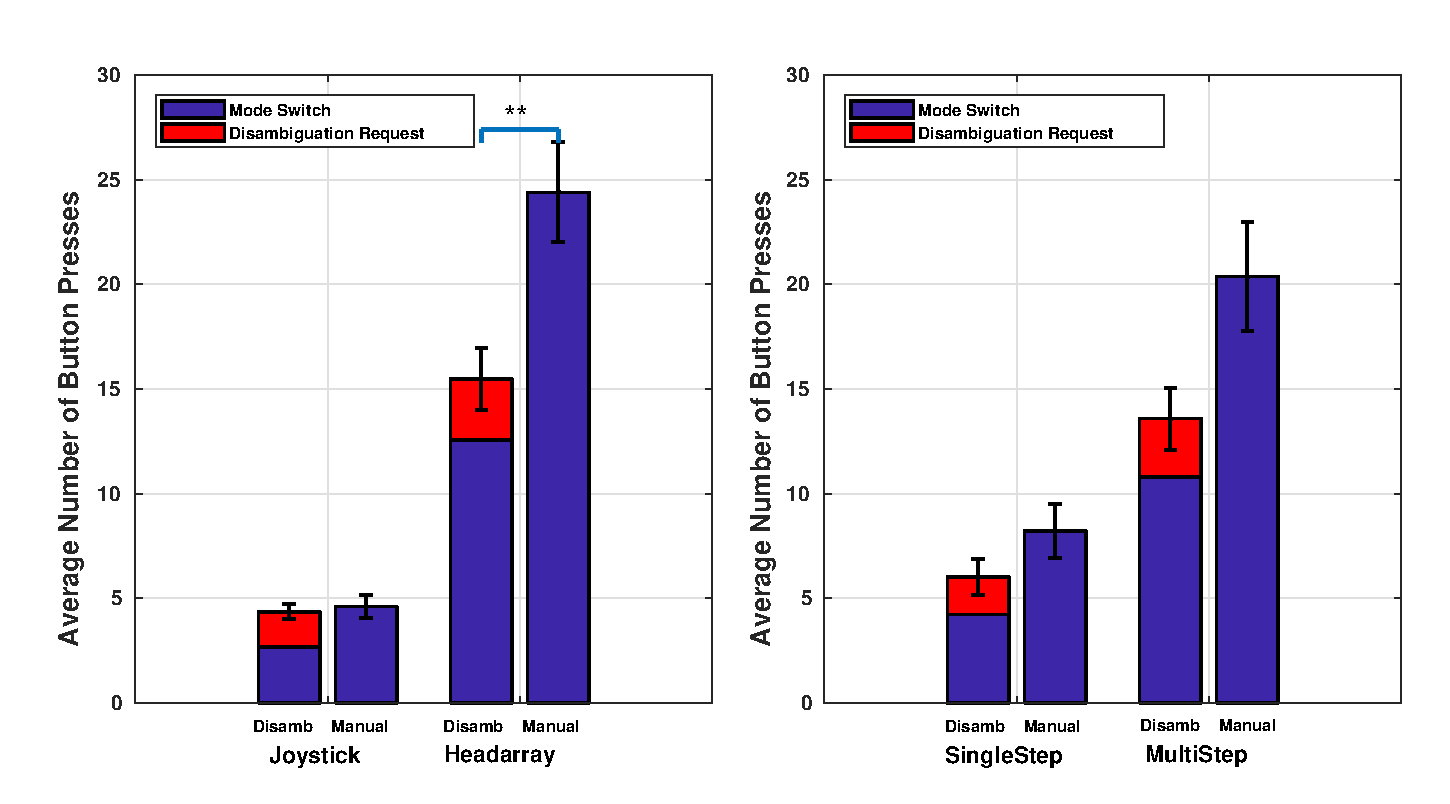
\includegraphics[keepaspectratio, width = 0.91\hsize ,center]{Fig8.eps}
	\caption{Comparison of average number of button presses between \textit{Disambiguation} and \textit{Manual} Paradigms. \textit{Left:} Grouped by control interfaces. \textit{Right:} Grouped by tasks.}
	\label{fig:button_press}
\end{figure*}
Here we report the results of our subject study. Statistical significance was determined by the Wilcoxon Rank-Sum test in where (***) indicates $p < 0.001$, (**) $p < 0.01$ and (*) $p < 0.05$. 

\subsection{Impact of Disambiguation on Task Performance}
Figure~\ref{fig:button_press} presents the number of button presses under each mode switching paradigm, for both interfaces and tasks. 

A statistically significant decrease in the number of button presses was observed between the \textit{Manual} and \textit{Disambiguation} paradigms when using the headarray (Figure~\ref{fig:button_press}, Left). Due to the low-dimensionality of headarray and cyclical nature of mode switching, the number of button presses required for task completion is inherently high. That the disambiguation paradigm was helpful in reducing the number of button presses likely is due to higher robot assistance in the disambiguating control mode and therefore reduced the need for subsequent user-initiated mode switches. 

For joystick, statistically significant differences were observed for the number of manual mode switches between the two paradigms ($p < 0.05$, not pictured in Figure~\ref{fig:button_press}). However, the gain due to the reduction of user-initiated mode switches was offset by the button presses that were required for disambiguation requests. 

A general trend (although not statistically significant) of a decrease in the number of button presses was also observed for the more complex multi-step task (Figure~\ref{fig:button_press}, Right). 

These results suggest that disambiguation is more useful as the control interface becomes more limited and the task becomes more complex.Intuitively, intent prediction becomes harder for the robot when the control interface is low-dimensional and does not reveal a great deal about the user's underlying intent. By having the users operate the robot in the disambiguating mode, the robot is able to elicit more intent-expressive control commands from the human which in turn helps in accurate goal inference and subsequently appropriate robot assistance. 
\begin{table}[t]
	\centering
	\caption{Characterization of the temporal distribution of disambiguation requests. The values in the table denote the deviation of the temporal distribution from a uniform distribution. Smaller values mean more concentrated and earlier disambiguation requests. } 
%	\vspace{0.1cm}
	\label{table:skewness}
	\begin{tabular}{|c|c|c|c|}
		\hline
		& Single Step & Multi Step \\
		\hline
		Joystick & 0.63 & 0.57 \\
		\hline
		Headarray & 0.35 & 0.22 \\
		\hline
	\end{tabular}
\end{table}
\subsection{Temporal Distribution of Disambiguation Requests}
\begin{figure*}[ht!]
	\centering
	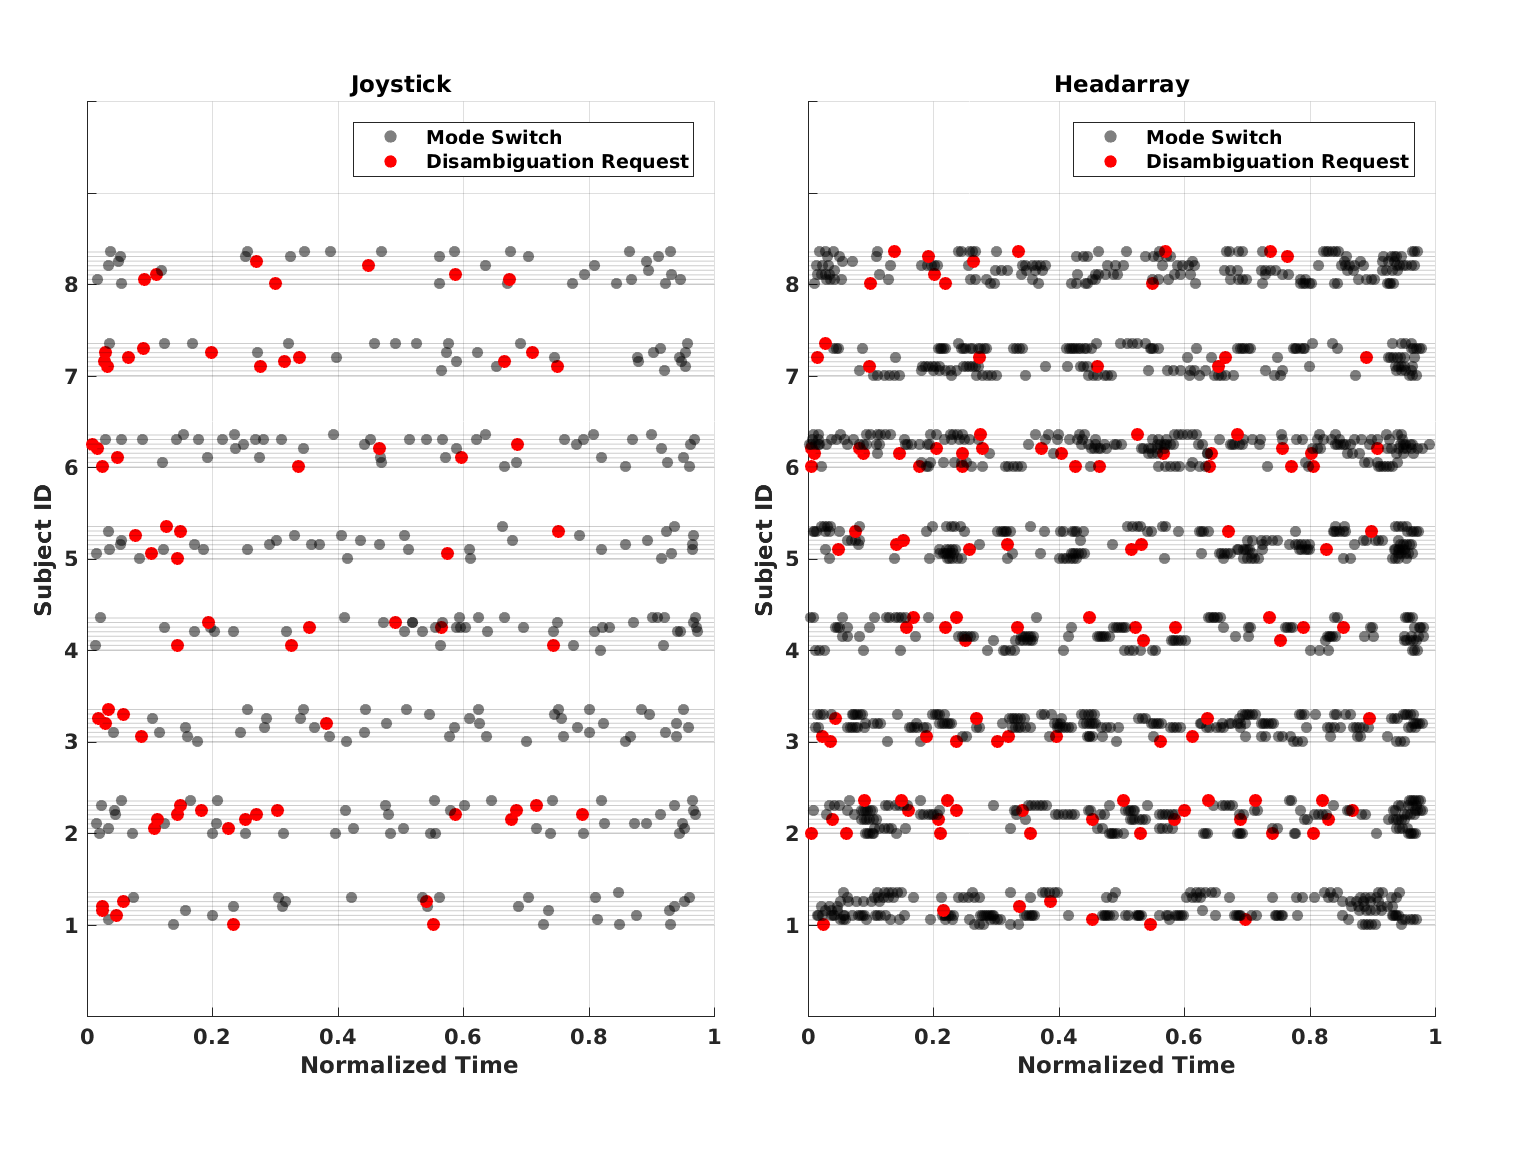
\includegraphics[width = 0.84\textwidth,center]{Fig9.eps}
	\caption{Temporal pattern of button presses for each interface and the multi-step task on a trial-by-trial basis for all subjects. Eight trials per subject per interface/task combination.}
	\label{fig:ha_man_disamb}
\end{figure*}
We also observed similar trends in the \textit{temporal distribution} of disambiguation requests, where a higher number of disambiguation requests correlates with the more limited interface and complex task. The temporal distribution of disambiguation requests refers to \textit{when} the subject requested assistance during the course of a trial. We use a measure of \textit{skewness} to characterize how much the temporal distribution deviates from a uniform distribution.\footnote{A uniform temporal distribution corresponds to a trial in which the disambiguation requests are uniformly spread out during the course of task execution. The skewness of a uniform distribution is $0$.} Larger positive values of skewness correlate with more concentrated and earlier disambiguation requests. Earlier disambiguation requests is possibly due to the fact that the subjects wanted progress towards the goal to happen right at the start of the trial itself. Table~\ref{table:skewness} reports the skewness of the temporal distribution of disambiguation requests for different interface-task combinations.


Figure~\ref{fig:ha_man_disamb} shows the temporal pattern of disambiguation requests and mode switches for the multi-step task on a trial-by-trial basis for all subjects. From the figure it is clear that the frequency and density of button presses (disambiguation requests plus mode switches) are much higher for the more limited control interface. The subjects also demonstrated a diverse range of disambiguation request behavior, for example in regards to both when during the execution requests were made and with what frequency (e.g. Subject 8 versus Subject 2, Joystick). The variation between subjects is likely due to different factors such as the user's comfort in operating the robot and understanding the ability of the disambiguating mode to recruit more assistance from the autonomy.


\subsection{Onset of Robot Assistance}\label{ssec:onset}
One of the motivations for developing the disambiguation system was that more accurate intent inference (as a result of intent disambiguation) should allow the autonomy to step in earlier more during the course of task execution. However, our results did not reveal any differences between the two switching paradigms across tasks or across interfaces (Figure~\ref{fig:initial_blend}). 
\begin{figure}[h!]
	\centering
	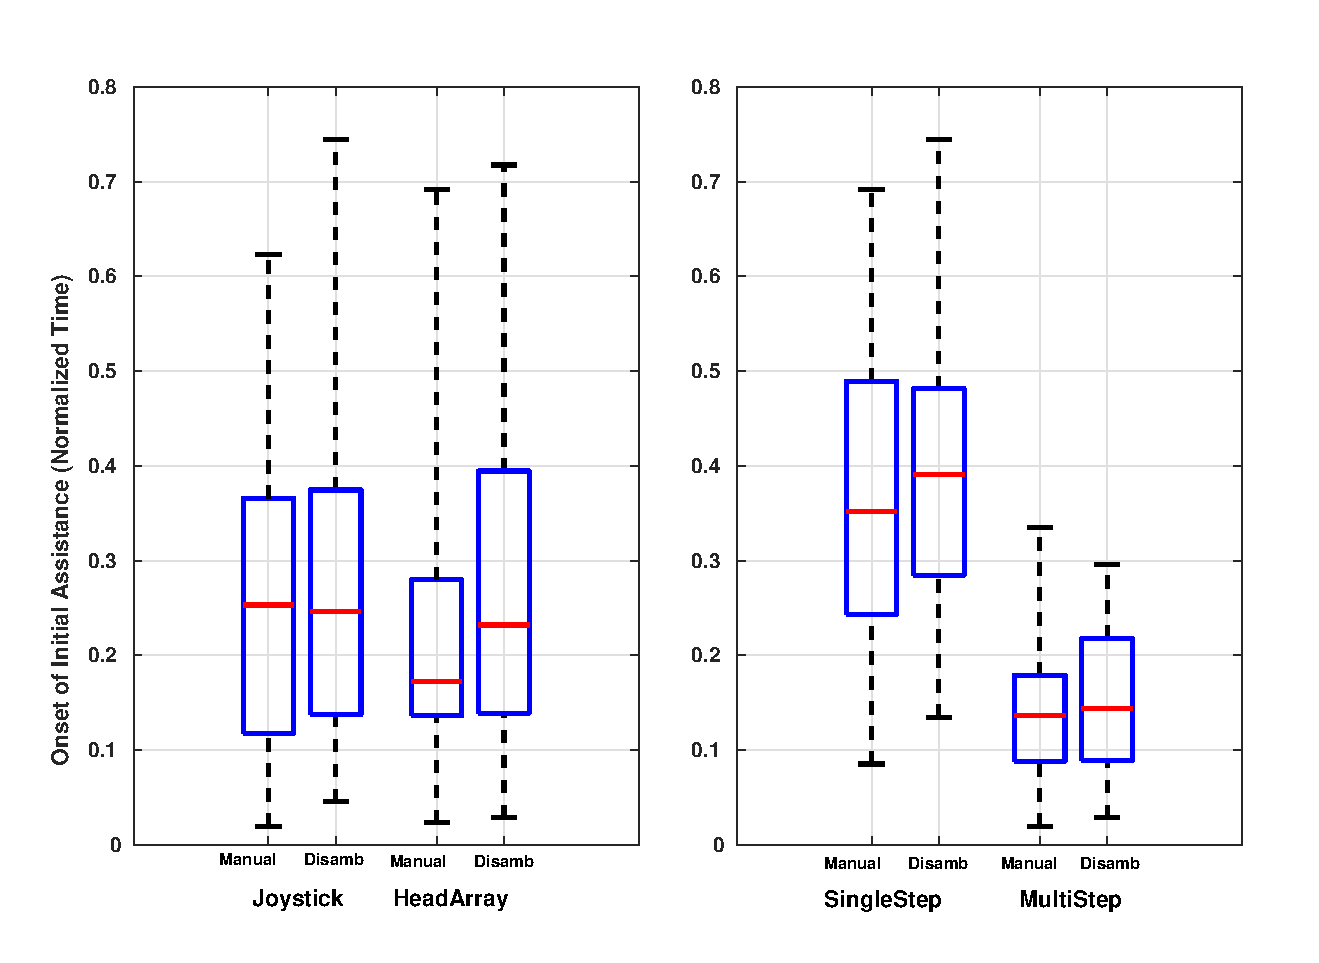
\includegraphics[width = 1\hsize ,center]{Fig11.eps}
	\caption{Onset of robot assistance normalized with respect to task completion time. \textit{Left:} Across interfaces. \textit{Right:} Across tasks.}
	\label{fig:initial_blend}
\end{figure}

\begin{figure*}[ht!]
	\centering
	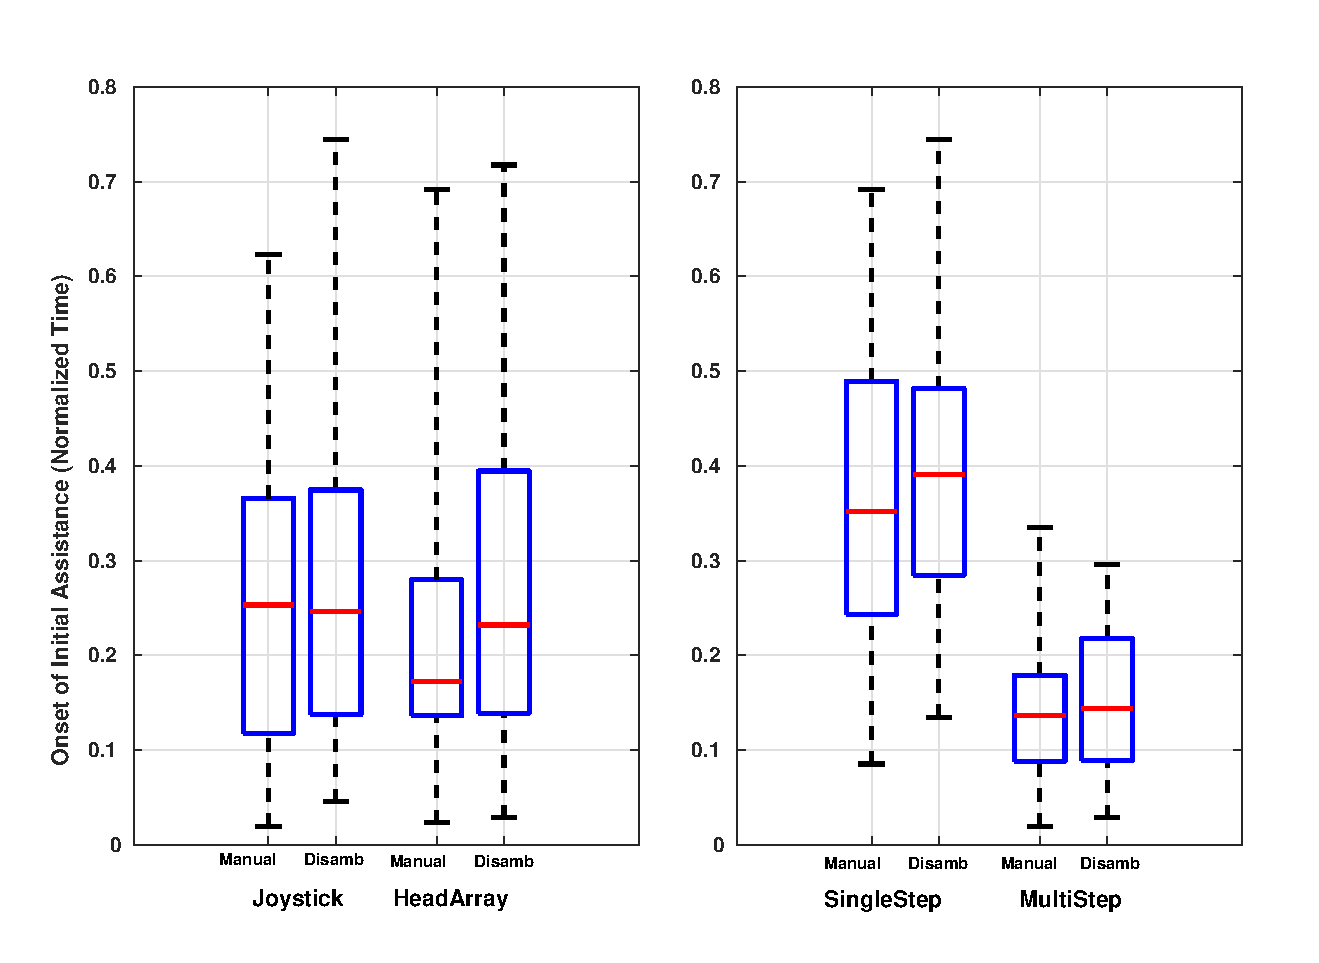
\includegraphics[width = 0.8\hsize, ,center]{Fig10.eps}
	\caption{Time evolution of goal probabilities. \textit{Top:} Multi-step task. \textit{Bottom:} Single-step task. The gray horizontal line above denotes the minimum threshold for robot assistance. The black bars at the bottom denote non-zero human control commands. The red and black dots indicate button presses that are disambiguation requests and mode switches respectively. }
	\label{fig:gp_evolution}
\end{figure*}


One likely contributing factor is that disambiguation frequently was impaired by subjects choosing not to operate in the disambiguation mode after making a disambiguation request. The disambiguation power of a control mode depends entirely on the observation of motion within that mode, and so in such scenarios disambiguation is effectively rendered inert.

This phenomenon is illustrated in Figure~\ref{fig:gp_evolution}. When control commands are issued, they are indicated by the black bars on the bottom of the plots. Disambiguation requests are shown as red dots, and mode switches as black dots. In the right plot, we see multiple instances of disambiguation requests being followed by no control commands or only very brief control commands and as a result the robot does not receive enough \textit{intent-expressive} cues from the user and the goal probability barely crosses the threshold for providing autonomy assistance. However, in the left plot, operation in the disambiguating mode quickly elevates one goal probability above the threshold for providing autonomy assistance, and after the assistance kicks in the subject elects to stop issuing control commands.

\subsection{User Survey}

Users rated the utility value of the system fairly high (mean = $5.52 \pm 1.07$) indicating that the users thought that the control modes chosen by the system made task execution easier. Subjects on average also indicated that they liked operating the robot in the disambiguating control modes (mean $5.00 \pm 1.15$). A majority of subjects (6 of 8) also preferred the disambiguation paradigm to the manual scheme, possibly due to a reduction in task effort as a result of operating the robot in the disambiguating modes.  However, only 4 of 8 subjects considered the disambiguation system to be user-friendly. Likely reasons are that the fact that the user had to initiate the disambiguation request, and that the system was not transparent about \textit{how} their button press helped the robot figure out which goal. In the former case, n automated mode switching scheme might improve user satisfaction and friendliness; and in the latter, including transparency as an objective of in the training period.
%
\section{Discussion}\label{sec:discussions}
 
 \added{The disambiguation algorithm presented in our work can be utilized in any human-robot system in which there is a need to disambiguate between the different states a discrete hidden variable (for example, discrete set of goals in robotic manipulation, set of landmarks in navigation tasks) can assume. Our algorithm also assumes the existence of a discrete set of parameters (for example, control modes for robotic manipulation, natural language-based queries for navigation) that can help the intent inference mechanism to unambiguously converge to the correct inference. Although the disambiguation algorithm is task-agnostic, (it relies exclusively on the shape features of the probability distribution over the hidden variable), the disambiguation is only as good as the efficacy of the intent inference algorithm that is used for as specific task. Therefore, it becomes important that the choice of cost functions and domain-specific heuristics is appropriate for the task at hand. }
 

 In a \textit{help me, help you} type of human robot system, task execution becomes seamless and more efficient when there is a sound mutual understanding of how the other party operates. One observation from our subject study was how often participants submitted a disambiguation request, and then chose not to operate in the selected mode---effectively not letting the robot help them. This highlights the need for greater transparency in human-robot interaction so that the human has a clear picture of \textit{how} and \textit{why} the robot chooses to help the user in certain ways. A lack of understanding of how they might help the robot to help them might have resulted in the under-utilization of the disambiguation feature. In order to provide \textit{intent-expressive} control commands to the robot, very likely knowledge of the assistance mechanism is critical.  Important to note is that this work was not about having the system select a control mode that the \textit{human} wants to use to reach a target (which might be motivated by a wide variety of factors such as line of sight or ease of use). In spite of this, subject responses to the user survey indicated that majority of the subjects liked operating the robot in the disambiguating modes and felt that task execution became easier as a result. 
 
 Therefore, the need for extensive and thorough training becomes apparent.
 The training can be made more effective in a few different ways. First, online feedback of the robot's intent prediction at all times during training can likely help the subject gain a better understanding of the relationship between the characteristics of their control actions (sparsity, aggressiveness, persistence) and the robot's assistive behavior. Second, the subjects could be explicitly informed of the task relevant features (directedness, proximity \textit{et cetera}) that the robot relies on for determining the amount of assistance. Knowledge of these features might motivate the users to leverage the disambiguating mode. 
 
 The inherent time delays associated with the computation of the disambiguating mode (approximately 2-2.5s) might have been a discouraging factor and a cause for user frustration. The algorithm could be used to pre-compute a large set of most informative modes for different parts of the workspace, for different goal configurations and for different priors ahead of time, which then might be used a lookup table during task execution. Furthermore, metamodeling techniques and machine learning tools can be used to learn generalizable models that will be effective in previously unseen goal configurations. 
 
 In the present system, there is task effort associated with requesting disambiguation assistance which can discourage the users from utilizing the paradigm. Automated mode switching schemes can possibly eliminate the need for button presses for disambiguation requests. 
 We also identify an opportunity to have adaptive assistance
 paradigms that explicitly take into account the characteristics of the user's control behavior. Some users are timid in their operation of the robot whereas some others are more aggressive and confident. Some are more comfortable operating the robot manually and do not seek assistance, whereas some others rely on assistance more frequently. Individual user characteristics could be extracted from training and be used for tuning the parameters of the intent inference engine and the shared control system to maximize robustness and efficacy of the assistive system. This would also likely improve user satisfaction and result in higher user acceptance.
  

\section{Conclusion}\label{sec:conclusions}
In this paper, we have presented an algorithm for \textit{intent disambiguation assistance} with a shared-control robotic arm using the notion of \textit{inverse legibility}. The goal of our algorithm is to elicit more \textit{intent-expressive} control commands from the user by placing control in those control modes that \textit{maximally disambiguate} between the various goals in the scene. As a secondary contribution, we also present a novel intent inference mechanism inspired by \textit{dynamic field theory} that works in conjunction with the disambiguation system. Pilot user study was conducted with eight subjects to evaluate the efficacy of the disambiguation system. Our results indicate a decrease in task effort in terms of the number of button presses when disambiguation system employed. 

In our future work, as informed by our pilot study, we plan to extend the framework into an automated mode switch assistance system. A more extensive user study with motor-impaired subjects will also be conducted in the future to further evaluate the utility of the disambiguation system and explore the disambiguation request patterns of users.  

%% For one-column wide figures use
%\begin{figure}
%% Use the relevant command to insert your figure file.
%% For example, with the graphicx package use
%  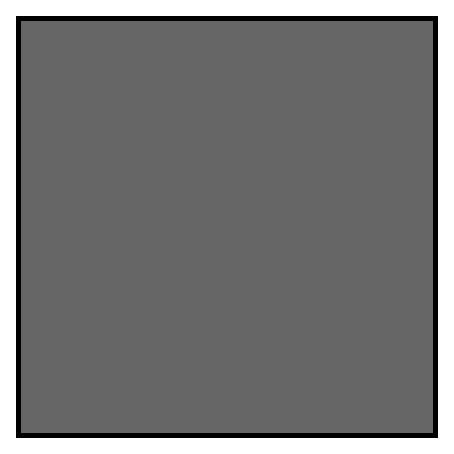
\includegraphics{example.eps}
%% figure caption is below the figure
%\caption{Figure1}
%\label{fig:1}       % Give a unique label
%\end{figure}
%%
%% For two-column wide figures use
%\begin{figure*}
%% Use the relevant command to insert your figure file.
%% For example, with the graphicx package use
%  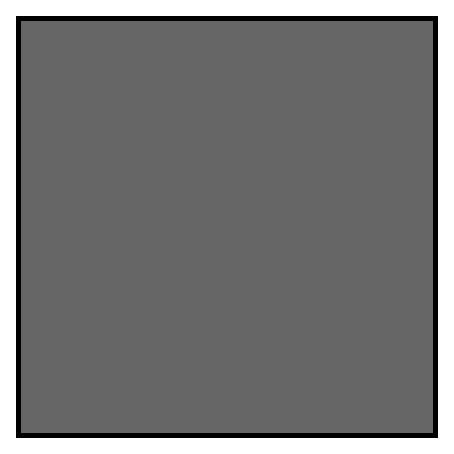
\includegraphics[width=0.75\textwidth]{example.eps}
%% figure caption is below the figure
%\caption{Figure2}
%\label{fig:2}       % Give a unique label
%\end{figure*}
%%
%% For tables use
%\begin{table}[h!]
%% table caption is above the table
%\caption{Please write your table caption here}
%\label{tab:1}       % Give a unique label
%% For LaTeX tables use
%\begin{tabular}{lll}
%\hline\noalign{\smallskip}
%first & second & third  \\
%\noalign{\smallskip}\hline\noalign{\smallskip}
%number & number & number \\
%number & number & number \\
%\noalign{\smallskip}\hline
%\end{tabular}
%\end{table}

% BibTeX users please use one of
\balance
\bibliographystyle{spbasic}      % basic style, author-year citations
%\bibliographystyle{spmpsci}      % mathematics and physical sciences
%\bibliographystyle{spphys}       % APS-like style for physics
\bibliography{references.bib}   % name your BibTeX data base

% Non-BibTeX users please use
%\begin{thebibliography}{}
%%
%% and use \bibitem to create references. Consult the Instructions
%% for authors for reference list style.
%%
%\bibitem{RefJ}
%% Format for Journal Reference
%Author, Article title, Journal, Volume, page numbers (year)
%% Format for books
%\bibitem{RefB}
%Author, Book title, page numbers. Publisher, place (year)
%% etc
%\end{thebibliography}
%\begin{thebibliography}{54}
%	\providecommand{\natexlab}[1]{#1}
%	\providecommand{\url}[1]{{#1}}
%	\providecommand{\urlprefix}{URL }
%	\expandafter\ifx\csname urlstyle\endcsname\relax
%	\providecommand{\doi}[1]{DOI~\discretionary{}{}{}#1}\else
%	\providecommand{\doi}{DOI~\discretionary{}{}{}\begingroup
%		\urlstyle{rm}\Url}\fi
%	\providecommand{\eprint}[2][]{\url{#2}}
%	
%	\bibitem[{Amari(1977)}]{amari1977dynamics}
%	Amari Si (1977) Dynamics of pattern formation in lateral-inhibition type neural
%	fields. \textit{Biological Cybernetics} 27(2):77--87
%	
%	
%	\bibitem[{Argall et~al(2009)Argall, Chernova, Veloso, and
%		Browning}]{argall2009survey}
%	Argall BD, Chernova S, Veloso M, Browning B (2009) A survey of robot learning
%	from demonstration. \textit{Robotics and Autonomous Systems} 57(5):469--483
%	
%	\bibitem[{Atanasov et~al(2014)Atanasov, Le~Ny, Daniilidis, and
%		Pappas}]{atanasov2014information}
%	Atanasov N, Le~Ny J, Daniilidis K, Pappas GJ (2014) Information acquisition
%	with sensing robots: Algorithms and error bounds. In: \textit{Proceedings of
%		the IEEE International Conference on Robotics and Automation (ICRA)}
%	
%	\bibitem[{Baker et~al(2007)Baker, Tenenbaum, and Saxe}]{baker2007goal}
%	Baker CL, Tenenbaum JB, Saxe RR (2007) Goal inference as inverse planning. In:
%	\textit{Proceedings of the Cognitive Science Society}
%	
%	\bibitem[{Baker et~al(2009)Baker, Saxe, and Tenenbaum}]{baker2009action}
%	Baker CL, Saxe RR, Tenenbaum JB (2009) Action understanding as inverse
%	planning. \textit{Cognition} 113(3):329--349
%	
%	\bibitem[{Choi et~al(2008)Choi, Anderson, Glass, and Kemp}]{choi2008laser}
%	Choi YS, Anderson CD, Glass JD, Kemp CC (2008) Laser pointers and a touch
%	screen: intuitive interfaces for autonomous mobile manipulation for the motor
%	impaired. In: \textit{Proceedings of the International SIGACCESS Conference
%		on Computers and Accessibility}
%	
%	\bibitem[{Demeester et~al(2008)Demeester, H{\"u}ntemann, Vanhooydonck,
%		Vanacker, Van~Brussel, and Nuttin}]{demeester2008user}
%	Demeester E, H{\"u}ntemann A, Vanhooydonck D, Vanacker G, Van~Brussel H, Nuttin
%	M (2008) User-adapted plan recognition and user-adapted shared control: A
%	bayesian approach to semi-autonomous wheelchair driving. \textit{Autonomous
%		Robots} 24(2):193--211
%	
%	\bibitem[{Downey et~al(2016)Downey, Weiss, Muelling, Venkatraman, Valois,
%		Hebert, Bagnell, Schwartz, and Collinger}]{downey2016blending}
%	Downey JE, Weiss JM, Muelling K, Venkatraman A, Valois JS, Hebert M, Bagnell
%	JA, Schwartz AB, Collinger JL (2016) Blending of brain-machine interface and
%	vision-guided autonomous robotics improves neuroprosthetic arm performance
%	during grasping. \textit{Journal of Neuroengineering and Rehabilitation}
%	13(1):28
%	
%	\bibitem[{Dragan and Srinivasa(2012)}]{dragan2012assistive}
%	Dragan AD, Srinivasa SS (2012) Assistive teleoperation for manipulation tasks.
%	In: \textit{Proceedings of ACM/IEEE International Conference on Human-Robot
%		Interaction (HRI)}
%	
%	\bibitem[{Dragan et~al(2013)Dragan, Lee, and Srinivasa}]{dragan2013legibility}
%	Dragan AD, Lee KC, Srinivasa SS (2013) Legibility and predictability of robot
%	motion. In: \textit{Proceedings of the ACM/IEEE International Conference on
%		Human-Robot Interaction (HRI)}
%	
%	\bibitem[{Driessen et~al(2005)Driessen, Kate, Liefhebber, Versluis, and
%		Van~Woerden}]{driessen2005collaborative}
%	Driessen B, Kate TT, Liefhebber F, Versluis A, Van~Woerden J (2005)
%	Collaborative control of the manus manipulator. \textit{Universal Access in
%		the Information Society} 4(2):165--173
%	
%	\bibitem[{Eftring and Boschian(1999)}]{eftring1999technical}
%	Eftring H, Boschian K (1999) Technical results from manus user trials. In:
%	\textit{IEEE 2nd International Conference on Rehabilitation Robotics (ICORR)}
%	
%	\bibitem[{Erlhagen and Bicho(2006)}]{erlhagen2006dynamic}
%	Erlhagen W, Bicho E (2006) The dynamic neural field approach to cognitive
%	robotics. \textit{Journal of Neural Engineering} 3(3):R36
%	
%	\bibitem[{Erlhagen and Bicho(2014)}]{erlhagen2014dynamic}
%	Erlhagen W, Bicho E (2014) A dynamic neural field approach to natural and
%	efficient human-robot collaboration. In: \textit{Neural Fields}, Springer, pp
%	341--365
%	
%	\bibitem[{Faubel and Sch{\"o}ner(2008)}]{faubel2008learning}
%	Faubel C, Sch{\"o}ner G (2008) Learning to recognize objects on the fly: a
%	neurally based dynamic field approach. \textit{Neural Networks}
%	21(4):562--576
%	
%	\bibitem[{Goodfellow et~al(2010)Goodfellow, Koenig, Muja, Pantofaru, Sorokin,
%		and Takayama}]{goodfellow2010help}
%	Goodfellow IJ, Koenig N, Muja M, Pantofaru C, Sorokin A, Takayama L (2010) Help
%	me help you: Interfaces for personal robots. In: \textit{Proceedings of
%		ACM/IEEE International Conference on Human-Robot Interaction (HRI)}
%	
%	\bibitem[{Gopinath and Argall(2017)}]{gopinath2017mode}
%	Gopinath D, Argall B (2017) Mode switch assistance to maximize human intent
%	disambiguation. In: \textit{Robotics: Science and Systems}
%	
%	\bibitem[{Gopinath et~al(2017)Gopinath, Jain, and Argall}]{gopinath2017human}
%	Gopinath D, Jain S, Argall BD (2017) Human-in-the-loop optimization of shared
%	autonomy in assistive robotics. \textit{IEEE Robotics and Automation Letters}
%	2(1):247--254
%	
%	\bibitem[{Herlant et~al(2016)Herlant, Holladay, and
%		Srinivasa}]{herlant2016assistive}
%	Herlant LV, Holladay RM, Srinivasa SS (2016) Assistive teleoperation of robot
%	arms via automatic time-optimal mode switching. In: \textit{Proceedings of
%		the ACM/IEEE International Conference on Human-Robot Interaction (HRI)}
%	
%	\bibitem[{Holladay et~al(2014)Holladay, Dragan, and
%		Srinivasa}]{holladay2014legible}
%	Holladay RM, Dragan AD, Srinivasa SS (2014) Legible robot pointing. In:
%	\textit{The IEEE International Symposium on Robot and Human Interactive
%		Communication (RO-MAN)}
%	
%	\bibitem[{Hsu et~al(2002)Hsu, Kindel, Latombe, and Rock}]{hsu2002randomized}
%	Hsu D, Kindel R, Latombe JC, Rock S (2002) Randomized kinodynamic motion
%	planning with moving obstacles. \textit{The International Journal of Robotics
%		Research} 21(3):233--255
%	
%	\bibitem[{Huete et~al(2012)Huete, Victores, Martinez, Gim{\'e}nez, and
%		Balaguer}]{huete2012personal}
%	Huete AJ, Victores JG, Martinez S, Gim{\'e}nez A, Balaguer C (2012) Personal
%	autonomy rehabilitation in home environments by a portable assistive robot.
%	\textit{IEEE Transactions on Systems, Man, and Cybernetics, Part C
%		(Applications and Reviews)} 42(4):561--570
%	
%	\bibitem[{Kelley et~al(2008)Kelley, Tavakkoli, King, Nicolescu, Nicolescu, and
%		Bebis}]{kelley2008understanding}
%	Kelley R, Tavakkoli A, King C, Nicolescu M, Nicolescu M, Bebis G (2008)
%	Understanding human intentions via hidden markov models in autonomous mobile
%	robots. In: \textit{Proceedings of the 3rd ACM/IEEE International Conference
%		on Human Robot Interaction}, ACM, pp 367--374
%	
%	\bibitem[{Khatib(1986)}]{khatib1986real}
%	Khatib O (1986) Real-time obstacle avoidance for manipulators and mobile
%	robots. \textit{The International Journal of Robotics Research} 5(1):90--98
%	
%	\bibitem[{Kim et~al(2010)Kim, Hazlett, Godfrey, Rucks, Portee, Bricout,
%		Cunningham, and Behal}]{kim2010relationship}
%	Kim DJ, Hazlett R, Godfrey H, Rucks G, Portee D, Bricout J, Cunningham T, Behal
%	A (2010) On the relationship between autonomy, performance, and satisfaction:
%	Lessons from a three-week user study with post-sci patients using a smart
%	6dof assistive robotic manipulator. In: \textit{Proceeding of the IEEE
%		International Conference on Robotics and Automation (ICRA)}, IEEE, pp
%	217--222
%	
%	\bibitem[{Kim et~al(2012)Kim, Hazlett-Knudsen, Culver-Godfrey, Rucks,
%		Cunningham, Portee, Bricout, Wang, and Behal}]{kim2012autonomy}
%	Kim DJ, Hazlett-Knudsen R, Culver-Godfrey H, Rucks G, Cunningham T, Portee D,
%	Bricout J, Wang Z, Behal A (2012) How autonomy impacts performance and
%	satisfaction: Results from a study with spinal cord injured subjects using an
%	assistive robot. \textit{IEEE Transactions on Systems, Man, and
%		Cybernetics-Part A: Systems and Humans} 42(1):2--14
%	
%	\bibitem[{LaPlante et~al(1992)}]{laplante1992assistive}
%	LaPlante MP, et~al (1992) Assistive technology devices and home accessibility
%	features: prevalence, payment, need, and trends. \textit{Advance Data from
%		Vital and Health Statistics}
%	
%	\bibitem[{Liu et~al(2016)Liu, Hamrick, Fisac, Dragan, Hedrick, Sastry, and
%		Griffiths}]{liu2016goal}
%	Liu C, Hamrick JB, Fisac JF, Dragan AD, Hedrick JK, Sastry SS, Griffiths TL
%	(2016) Goal inference improves objective and perceived performance in
%	human-robot collaboration. In: \textit{Proceedings of the 2016 International
%		Conference on Autonomous Agents \& Multiagent Systems}, International
%	Foundation for Autonomous Agents and Multiagent Systems, pp 940--948
%	
%	\bibitem[{Miller and Murphey(2013)}]{miller2013trajectory}
%	Miller LM, Murphey TD (2013) Trajectory optimization for continuous ergodic
%	exploration. In: \textit{American Control Conference (ACC)}
%	
%	\bibitem[{Miller et~al(2016)Miller, Silverman, MacIver, and
%		Murphey}]{miller2016ergodic}
%	Miller LM, Silverman Y, MacIver MA, Murphey TD (2016) Ergodic exploration of
%	distributed information. \textit{IEEE Transactions on Robotics} 32(1):36--52
%	
%	\bibitem[{Muelling et~al(2017)Muelling, Venkatraman, Valois, Downey, Weiss,
%		Javdani, Hebert, Schwartz, Collinger, and Bagnell}]{muelling2017autonomy}
%	Muelling K, Venkatraman A, Valois JS, Downey JE, Weiss J, Javdani S, Hebert M,
%	Schwartz AB, Collinger JL, Bagnell JA (2017) Autonomy infused teleoperation
%	with application to brain computer interface controlled manipulation.
%	\textit{Autonomous Robots} pp 1--22
%	
%	\bibitem[{Nuttin et~al(2002)Nuttin, Vanhooydonck, Demeester, and
%		Van~Brussel}]{nuttin2002selection}
%	Nuttin M, Vanhooydonck D, Demeester E, Van~Brussel H (2002) Selection of
%	suitable human-robot interaction techniques for intelligent wheelchairs. In:
%	\textit{Proceedings of 11th IEEE International Workshop on Robot and Human
%		Interactive Communication}, IEEE, pp 146--151
%	
%	\bibitem[{Philips et~al(2007)Philips, Mill{\'a}n, Vanacker, Lew, Gal{\'a}n,
%		Ferrez, Van~Brussel, and Nuttin}]{philips2007adaptive}
%	Philips J, Mill{\'a}n JdR, Vanacker G, Lew E, Gal{\'a}n F, Ferrez PW,
%	Van~Brussel H, Nuttin M (2007) Adaptive shared control of a brain-actuated
%	simulated wheelchair. In: \textit{Proceedings of the IEEE International
%		Conference on Rehabilitation Robotics (ICORR)}, IEEE, pp 408--414
%	
%	\bibitem[{Pilarski et~al(2012)Pilarski, Dawson, Degris, Carey, and
%		Sutton}]{pilarski2012dynamic}
%	Pilarski PM, Dawson MR, Degris T, Carey JP, Sutton RS (2012) Dynamic switching
%	and real-time machine learning for improved human control of assistive
%	biomedical robots. In: \textit{Proceedings of the IEEE RAS \& EMBS
%		International Conference on Biomedical Robotics and Biomechatronics (BioRob)
%	}, IEEE, pp 296--302
%	
%	\bibitem[{Ratliff et~al(2009)Ratliff, Zucker, Bagnell, and
%		Srinivasa}]{ratliff2009chomp}
%	Ratliff N, Zucker M, Bagnell JA, Srinivasa S (2009) Chomp: Gradient
%	optimization techniques for efficient motion planning. In:
%	\textit{Proceedings of the IEEE International Conference on Robotics and
%		Automation (ICRA)}, IEEE, pp 489--494
%	
%	\bibitem[{Rimon and Koditschek(1992)}]{rimon1992exact}
%	Rimon E, Koditschek DE (1992) Exact robot navigation using artificial potential
%	functions. \textit{IEEE Transactions on Robotics and Automation}
%	8(5):501--518
%	
%	\bibitem[{Sadigh et~al(2016{\natexlab{a}})Sadigh, Sastry, Seshia, and
%		Dragan}]{sadigh2016planning}
%	Sadigh D, Sastry S, Seshia SA, Dragan AD (2016{\natexlab{a}}) Planning for
%	autonomous cars that leverage effects on human actions. In: \textit{Robotics:
%		Science and Systems}
%	
%	\bibitem[{Sadigh et~al(2016{\natexlab{b}})Sadigh, Sastry, Seshia, and
%		Dragan}]{sadigh2016information}
%	Sadigh D, Sastry SS, Seshia SA, Dragan A (2016{\natexlab{b}}) Information
%	gathering actions over human internal state. In: \textit{Proceedings of the
%		IEEE/RSJ International Conference on Intelligent Robots and Systems (IROS)},
%	IEEE, pp 66--73
%	
%	\bibitem[{Schaal(1997)}]{schaal1997learning}
%	Schaal S (1997) Learning from demonstration. In: \textit{Advances in Neural
%		Information Processing Systems}, pp 1040--1046
%	
%	\bibitem[{Scherer(1996)}]{scherer1996outcomes}
%	Scherer MJ (1996) Outcomes of assistive technology use on quality of life.
%	\textit{Disability and Rehabilitation} 18(9):439--448
%	
%	\bibitem[{Sch{\"o}ner(2008)}]{schoner2008dynamical}
%	Sch{\"o}ner G (2008) Dynamical systems approaches to cognition.
%	\textit{Cambridge Handbook of Computational Cognitive Modeling} pp 101--126
%	
%	\bibitem[{Sch{\"o}ner and Spencer(2015)}]{schoner2015dynamic}
%	Sch{\"o}ner G, Spencer J (2015) \textit{Dynamic thinking: A primer on dynamic
%		field theory}. Oxford University Press
%	
%	\bibitem[{Sch{\"o}ner et~al(1995)Sch{\"o}ner, Dose, and
%		Engels}]{schoner1995dynamics}
%	Sch{\"o}ner G, Dose M, Engels C (1995) Dynamics of behavior: Theory and
%	applications for autonomous robot architectures. \textit{Robotics and
%		Autonomous Systems} 16(2-4):213--245
%	
%	\bibitem[{Simpson et~al(2008)Simpson, Broughton, Gauthier, and
%		Prochazka}]{simpson2008tooth}
%	Simpson T, Broughton C, Gauthier MJ, Prochazka A (2008) Tooth-click control of a hands-free computer interface. \textit{IEEE Transactions on Biomedical Engineering} 55(8):2050--2056
%	
%	\bibitem[{Sorokin et~al(2010)Sorokin, Berenson, Srinivasa, and
%		Hebert}]{sorokin2010people}
%	Sorokin A, Berenson D, Srinivasa SS, Hebert M (2010) People helping robots
%	helping people: Crowdsourcing for grasping novel objects. In:
%	\textit{Proceedings of the IEEE/RSJ International Conference on Intelligent
%		Robots and Systems (IROS)}
%	
%	\bibitem[{Storms and Tilbury(2014)}]{storms2014blending}
%	Storms JG, Tilbury DM (2014) Blending of human and obstacle avoidance control
%	for a high speed mobile robot. In: \textit{American Control Conference
%		(ACC)}, IEEE, pp 3488--3493
%	
%	\bibitem[{Taha et~al(2011)Taha, Mir{\'o}, and Dissanayake}]{taha2011pomdp}
%	Taha T, Mir{\'o} JV, Dissanayake G (2011) A pomdp framework for modelling human
%	interaction with assistive robots. In: \textit{Proceedings of the IEEE
%		International Conference on Robotics and Automation (ICRA)}, IEEE, pp
%	544--549
%	
%	\bibitem[{Tanner et~al(2003)Tanner, Loizou, and
%		Kyriakopoulos}]{tanner2003nonholonomic}
%	Tanner HG, Loizou SG, Kyriakopoulos KJ (2003) Nonholonomic navigation and
%	control of cooperating mobile manipulators. \textit{IEEE Transactions on
%		Robotics and Automation} 19(1):53--64
%	
%	\bibitem[{Tomasello and Carpenter(2007)}]{tomasello2007shared}
%	Tomasello M, Carpenter M (2007) Shared intentionality. \textit{Developmental
%		Science} 10(1):121--125
%	
%	\bibitem[{Tomasello and Moll(2010)}]{tomasello2010gap}
%	Tomasello M, Moll H (2010) The gap is social: Human shared intentionality and
%	culture. In: \textit{Mind the Gap}, Springer, pp 331--349
%	
%	\bibitem[{Tsui et~al(2011)Tsui, Kim, Behal, Kontak, and Yanco}]{tsui2011want}
%	Tsui KM, Kim DJ, Behal A, Kontak D, Yanco HA (2011) “{I} want that”:
%	Human-in-the-loop control of a wheelchair-mounted robotic arm.
%	\textit{Applied Bionics and Biomechanics} 8(1):127--147
%	
%	\bibitem[{Wang et~al(2013)Wang, M{\"u}lling, Deisenroth, Ben~Amor, Vogt,
%		Sch{\"o}lkopf, and Peters}]{wang2013probabilistic}
%	Wang Z, M{\"u}lling K, Deisenroth MP, Ben~Amor H, Vogt D, Sch{\"o}lkopf B,
%	Peters J (2013) Probabilistic movement modeling for intention inference in
%	human--robot interaction. \textit{The International Journal of Robotics
%		Research} 32(7):841--858
%	
%	\bibitem[{Wilson and Cowan(1973)}]{wilson1973mathematical}
%	Wilson HR, Cowan JD (1973) A mathematical theory of the functional dynamics of
%	cortical and thalamic nervous tissue. \textit{Biological Cybernetics}
%	13(2):55--80
%	
%	\bibitem[{Zibner et~al(2011)Zibner, Faubel, Iossifidis, and
%		Schoner}]{zibner2011dynamic}
%	Zibner SK, Faubel C, Iossifidis I, Schoner G (2011) Dynamic neural fields as
%	building blocks of a cortex-inspired architecture for robotic scene
%	representation. \textit{IEEE Transactions on Autonomous Mental Development}
%	3(1):74--91
%	
%\end{thebibliography}
\end{document}
% end of file template.tex

